%\subsection{Historical review}

The early developments that led to the original MPM started with the \textbf{Particle-In-Cell} method (PIC) formulated for fluid dynamics problems \cite{PIC}. The novelty brought by PIC was the representation of a fluid by a collection of moving particles inside a background control volume subdivided into cells. Every single particle is given a constant mass and a position which is updated based on the velocity field resulting from the solution of linear momentum balance equation on the fixed background mesh. On the other hand, velocity, energy and pressure are stored at cells during the whole computation ($C^0$ approximation). A \textit{convective phase}, which consists in a weighting procedure, must be followed when a particle leaves a cell and enters a new one \cite{PIC}. Thus, the PIC enables the merging of Lagrangian and Eulerian techniques since the moving particles with ascribed masses enables the simulation of problems involving several highly deformed fluids without mesh distortion.

In spite of the good results provided by the PIC, the numerical diffusion it suffers from has been addressed by two different ways. First the method has been extended to a \textit{fully Lagrangian} approach \cite{McCrory_FLIP} by storing not only mass and position but all the fields at particles. Next, a new projection procedure has been proposed between the grid and the particles in order to reach second-order accuracy in space of the convective phase \cite{PIC_Nishiguchi}. The merging of those two improvements yielded the so-called \textbf{FLuid Implicit Particle} method (FLIP) \cite{FLIP}. In this new PIC formulation, every quantities are stored at particles so that the grid is only used for solving balance equations and hence provides an adaptive feature to the numerical scheme. The projection of fields from Lagrangian particles to the Eulerian mesh is made as in PIC while the backward mapping models the \textit{collisional} behavior of the fluid and leads to a double definition of the velocity. Indeed, the linear momentum resulting from the solution of balance equations on the grid is used to update the position of particles, whereas the change of linear momentum is used to update their velocity \cite{Mass_Flip}. This procedure yields a time derivative of particles displacement that is different from their velocity which, although it introduces oscillations in the vicinity of discontinuities, provides better results in terms of numerical diffusion \cite{Mass_Flip}.

Even though particles carry the whole history of the problem, FLIP has been essentialy used until the 90's to model history-independent constitutive models wich were dealt with on the grid. The first application of the method to history-dependent materials was made in the context of solid mechanics and yields the \textbf{Material Point Method} (MPM) \cite{Sulsky94}. %Since this formulation was based on a weak formulation for which \textit{material points} plays the role of integration points, the MPM may be seen as an extension of the Finite Element Method with moving Gauss points. Indeed, each material point is ascribed a volume by means of a delta Dirac \textit{characteristic function} which allows to approximate the volume integrals of the weak form by discrete sums over the Lagrangian particles.

\subsection{Derivation of the mpm}
Consider a solid domain with volume $\Omega_t$ bounded by the surface $\partial \Omega_t$, subject to traction forces and prescribed velocity on its boundaries within the time interval $\tau$:
\begin{align}
  & \tens{\sigma}\cdot\vect{n}=\vect{T}^d \quad \text{on } \partial \Omega_t^\sigma\\
  & \vect{v} = \vect{v}^d \quad \text{on } \partial \Omega_t^v
\end{align}
where $\vect{n}$ is the outward normal vector to $\partial \Omega_t$ and the set of boundaries satisfies $\partial \Omega_t =\partial \Omega^\sigma_t \cap \partial \Omega^v_t$.
%We seek an approximate solution of the eulerian balance equation of linear momentum \eqref{eq:HPP_linear_momentum} in a finite-dimensional function space using Galerkin approach. 

\subsubsection*{Weak formulation of the continuum problem}
The weak form of the eulerian balance equation of linear momentum \eqref{eq:HPP_linear_momentum} is written based on the Galerkin approach and the following function spaces:
\begin{equation}
\Vscr^1 = \{ \vect{u} \in H^1(\Omega_t) \}  \quad ; \quad \Vscr^1_{h} = \{\vect{u} \in \Vscr^1 | \vect{u}=\vect{v}^d \text{ on } \partial \Omega_t^v \}  \quad ; \quad \Vscr^1_{h,0} = \{\vect{u} \in \Vscr_h^1 | \vect{u}=\vect{0} \text{ on } \partial \Omega_t^v \} 
\end{equation}
where $H^1(\Omega_t)$ denotes the \textit{Sobolev} space in $\Omega_t$ \cite{DiPietro}. Thus, multiplication of equation \eqref{eq:HPP_linear_momentum} by a test function $\vect{w} \in \Vscr^1_{h,0}$ and integration over $\Omega_t$ yields, after integration by parts, the following weak form:
\begin{equation}
  \label{eq:linear_momentum_weak_form}
  \begin{aligned}
    &\text{Find $\vect{v}\in \Vscr_h^1$ such that} \\
    &\int_{\Omega_t}  \rho  \vect{\dot{v}} \cdot \vect{w}\: dv + \int_{\Omega_t}\tens{\sigma}: 
    \nablat \vect{w} \:dv - \int_{\partial \Omega^\sigma_t} \vect{T}^d\cdot\vect{w}\: ds= \int_{\Omega_t} \rho \vect{b}\cdot \vect{w} \: dv  \qquad \forall \: \vect{w} \in \Vscr_{h,0}^1
  \end{aligned}
\end{equation}

\subsubsection{The MPM discretization}
The continuum body is discretized into a set of $N_p$ material points in an arbitrary Cartesian grid. The grid is here supposed to be made of $N_n$ nodes and $E$ non-overlapping cells or elements, which set of faces separating cells that contain particles and having empty neighboring elements defines the boundary of the mesh (see figure \ref{fig:domain} for a two-dimensional case).
\begin{figure}[h!]
  \centering
  {\begin{tikzpicture}[scale=0.8]
  % \draw[step=1.0,black,thin] (-3.,-1.) grid (3,4.);
  \draw[white] (-3,-1) -- (3,-1) -- (3,4) -- (-3,4) -- (-3,-1);
  \begin{scope}[scale=0.5]
    \draw[thick] (-3,0.6) .. controls +(1,0) and +(-1,0) .. (0,1.8)  
    .. controls +(1,0) and +(0,-3) .. (5,3.2) 
    .. controls +(0,2) and +(2,0)  .. (0,5.2) 
    .. controls +(-1,0) and +(0,3) .. (-4.5,2.2) 
    .. controls +(0,-1) and +(-1,0).. (-3,0.6) ;
    \begin{scope}  % pour limiter la portée du clip
      \clip (-3,0.6) .. controls +(1,0) and +(-1,0) .. (0,1.8) 
      .. controls +(1,0) and +(0,-3) .. (5,3.2)
      .. controls +(0,2) and +(2,0)  .. (0,5.2)
      .. controls +(-1,0) and +(0,3) .. (-4.5,2.2)
      .. controls +(0,-1) and +(-1,0).. (-3,0.6);
    \end{scope}
    \node[below] at (0,1) {$\Omega_t$};
  \end{scope}
  \draw [->,very thick,gray] (3.,1.5) -- (3.6,1.5);
\end{tikzpicture}}
  {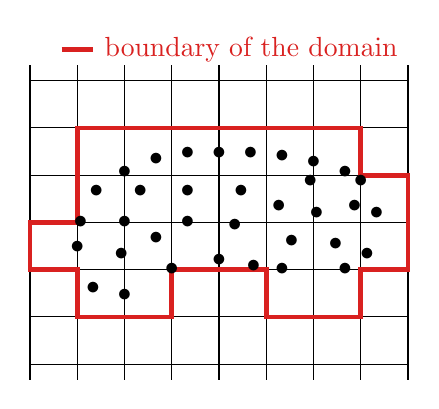
\begin{tikzpicture}[scale=0.8]
  \draw[step=.75,black,thin] (-3.,-1.) grid (3,4.);
  \draw[line width=0.6mm,Red] (-2.25,2.25) -- (-2.25,2.25)-- (-2.25,3)-- (2.25,3) --(2.25,2.25) -- (3.,2.25)-- (3.,0.75) --(2.25,0.75) --(2.25,0.) -- (0.75,0.) --(0.75,0.75) --(-0.75,0.75)-- (-0.75,0.)-- (-2.25,0.) -- (-2.25,0.75) --  (-3.,0.75)--(-3.,1.5) --(-2.25,1.5)--(-2.25,2.25);
  % contour
  \node at (0,0.9) {$\bullet$}  ; \node at (2.5,1.65) {$\bullet$}  ; 
  \node at (0,2.6) {$\bullet$}  ;\node at (-2.25,1.1) {$\bullet$}  ; 
  \node at (-1.5,0.35) {$\bullet$}  ; \node at (-2.,0.45) {$\bullet$}  ;
  \node at (-2.2,1.5) {$\bullet$}  ; \node at (-1.5,2.3) {$\bullet$}  ; 
  \node at (2.35,1.) {$\bullet$}  ; \node at (2.25,2.15) {$\bullet$}  ;
  \node at (0.55,0.8) {$\bullet$}  ; \node at (-0.5,2.6) {$\bullet$}  ; 
  \node at (0.5,2.59) {$\bullet$}  ; \node at (1.5,2.45) {$\bullet$}  ;
  \node at (1,0.75) {$\bullet$}; \node at (2,0.75) {$\bullet$}  ;
  \node at (2,2.3) {$\bullet$}  ; \node at (1,2.55) {$\bullet$}  ;
  \node at (-1,2.5) {$\bullet$}  ; \node at (-1.95,2.) {$\bullet$}  ;
  % interior
  \node at (-1.5,1.5) {$\bullet$}  ; \node at (-1.25,2.) {$\bullet$}  ;
  \node at (-0.75,0.75) {$\bullet$}  ; \node at (-1.55,1.) {$\bullet$}  ;
  \node at (-0.5,1.5) {$\bullet$}  ; \node at (-0.5,2.) {$\bullet$}  ;
  \node at (0.25,1.45) {$\bullet$}  ; \node at (0.35,2.) {$\bullet$}  ;
  \node at (0.95,1.75) {$\bullet$}  ; \node at (1.15,1.2) {$\bullet$}  ;
  \node at (1.45,2.15) {$\bullet$}  ; \node at (1.55,1.65) {$\bullet$}  ;
  \node at (1.85,1.15) {$\bullet$}  ; \node at (2.15,1.75) {$\bullet$}  ;
  \node at (-1.,1.25) {$\bullet$}  ;
  \draw[line width=0.6mm,Red] (-2.5,4.25) -- (-2.,4.25) node [right] {\text{boundary of the domain}};
\end{tikzpicture}}
  \caption{Representation of a continuum body by a set of material points in $\Rbb^2$.}
  \label{fig:domain}	
\end{figure}
Analogously to the Finite Element Method (FEM) \cite{Belytschko}, the velocity is approximated on the MPM background mesh by:
\begin{equation}
  \label{eq:approximation_basis}
  \vect{v}(\vect{x},t)=S_i(\vect{x})\vect{v}^{i}(t)
\end{equation}
where $\vect{v}^{i}$ is the velocity of the $i$th grid node, and $S_i(\vect{x})$ the (linear) shape function attached to it. One feature of the MPM is that the mass density is approximated on the grid based on the mass carried by each material point:
\begin{equation}
  \label{eq:density_approx}
  \rho\(\vect{x},t\)=\sum_{p=1}^{N_p} m_p \delta(\vect{x}_p-\vect{x})
\end{equation}
where the delta Dirac distribution $\delta$ is often referred to as the \textit{characteristic function} of material points, and $\vect{x}_p$ is the position of the $p$th particle. In what follows, the dependence on time will be omitted for simplicity and $p$ and $i$ or $j$ stand respectively for material points and nodes.

By introducing a specific Cauchy tensor $\rho \tens{\bar{\sigma}}=\tens{\sigma}$ and the approximation of mass density \eqref{eq:density_approx} in the weak form \eqref{eq:linear_momentum_weak_form}, the property of the delta Dirac distribution yields:
\begin{equation}
  \begin{aligned}
    &\text{Find $\vect{v}\in \Vscr_h^1$ such that} \\
    & \sum_{p=1}^{N_p} m_p  \[\vect{\dot{v}}(\vect{x}_p) \cdot \vect{w}(\vect{x}_p) + \tens{\bar{\sigma}}(\vect{x}_p):\nablat \vect{w}(\vect{x}_p) \]  = \sum_{p=1}^{N_p}m_p \vect{b}(\vect{x}_p)\cdot \vect{w}(\vect{x}_p) + \int_{\partial \Omega^\sigma_t} \vect{T}^d\cdot\vect{w}\: ds  \qquad \forall \: \vect{w} \in \Vscr_{h,0}^1
  \end{aligned}
\end{equation}
Then, with the approximation \eqref{eq:approximation_basis}, the weak form reads:
\begin{equation}
  \label{eq:mpm_discrete_weak}
    \begin{aligned}
      &\text{Find $\vect{v} \in \Vscr_h^1$ such that} \\
      & \vect{w}^j \sum_{p=1}^{N_p} m_p  \[ S_{jp} S_{ip} \vect{\dot{v}}^i + \nablav S_{jp} \cdot \tens{\bar{\sigma}}^p \]  =  \vect{w}^j\( \sum_{p=1}^{N_p}m_p S_{jp}\vect{b}^i  + \int_{\partial \Omega^\sigma_t} S_j(\vect{x})\vect{T}^d\: ds\)  \qquad \forall \: \vect{w} \in \Vscr_{h,0}^1
  \end{aligned}
\end{equation}
in which $S_{ip}=S_i(\vect{x}_p)$ and $\tens{\bar{\sigma}}^p=\tens{\bar{\sigma}}(\vect{x}_p)$. Next, the arbitrariness of the test function $\vect{w}$ yields the semi-discrete equation in matrix form:
\begin{equation}
  \label{eq:mpm_semi-discrete}
  m_{ji} \vect{\dot{v}}^i = \vect{f}_{int}^j + \vect{f}_{ext}^j 
\end{equation}
where the definition of the mass matrix $m_{ij}$ and the internal and external force vectors $\vect{f}_{int}^j $ and $\vect{f}_{ext}^j$ are:
\begin{subequations}
  \begin{alignat}{1}
    & m_{ij}= \sum_{p=1}^{N_p} m_p  S_{jp} S_{ip} \label{eq:mass_matrix}\\
    & \vect{f}_{int}^j = - \sum_{p=1}^{N_p} m_p \nablav S_{jp} \cdot \tens{\bar{\sigma}}^p \label{eq:int_forces}\\
    & \vect{f}_{ext}^j =\sum_{p=1}^{N_p}m_p S_{jp}\vect{b}^i  + \int_{\partial \Omega^\sigma_t} S_j(\vect{x})\vect{T}^d\: ds \label{eq:ext_forces}
  \end{alignat}
\end{subequations}
The system \eqref{eq:mpm_semi-discrete} can be solved for the nodal accelerations $\vect{\dot{v}}^i$, and advanced in time by using an explicit time discretization so that the nodal velocities can be updated. Hence, the time interval $\tau$ is discretized in $N_T$ sub-intervals of size $\Delta t^n$ such that $\sum_{n=1}^{N_T} \Delta t^n = T$ and time integration is performed with an explicit forward Euler algorithm leading to discrete equations:
\begin{equation}
  \label{eq:mpm_discrete}
  \frac{\vect{v}^{i,n+1}-\vect{v}^{i,n}}{\Delta t^n} = \vect{\dot{v}}^i
\end{equation}
where the superscripts $\bullet^{k,l}$ denote the time step $l$ at which the $k$th nodal field is evaluated. 

Note that in the weak form, the particles play the role of integration points so that the mass matrix depends on the positions of material points in the grid and must be computed at each time step. Hence, the MPM can be seen as an extension of the Finite Element Method with moving Gauss points. However, a consequence of this quadrature rule is that the consistent mass matrix $m_{ji}$ may be singular when only one material point lies in an element due to the reduced integration. The use of a linear combination of the diagonally lumped mass matrix $m^L_i=\sum_p S_{ip}m_p$ (positive-definite), and the constitent mass matrix (positive semi-definite) is then recommended \cite{Love}. Nevertheless, since no parameter value is prescribed for this combination, the lumped mass matrix is widely used in MPM simulations, though it introduces some dissipation of kinetic energy \cite{Mass_Flip}.  

Recall that the background grid inherited from FLIP is arbitrary and that the fields must be projected from particles to the nodes to solve the linear system \eqref{eq:mpm_discrete} and back so that the material points advect the solution. The first mapping step, required to build the discrete form,
aims at satify the conservation of linear momentum from particles to the grid:
\begin{equation}
  \label{eq:particles2nodes}
  m^{L,n}_i \vect{v}^{i,n} = \sum_{p=1}^{N_p} S_{ip}m_p \vect{v}^{p,n}
\end{equation}
to be solved for each $\vect{v}^i$. Once the nodal accelerations are calculeted for system \eqref{eq:mpm_semi-discrete}, the velocity of each material points is \textbf{updated} as:
\begin{equation}
  \label{eq:mp_velocity_update}
  \vect{v}^{p,n+1}= \vect{v}^{p,n}+ \Delta t\sum_{i=1}^{N_n} S_{ip}\vect{\dot{v}}^{i}
\end{equation}
while the updated nodal velocities resulting from the solution of \eqref{eq:mpm_discrete} are used to update the particles positions:
\begin{equation}
  \label{eq:position_update}
  \vect{x}^{p,n+1}=\vect{x}^{p,n} + \Delta t\sum_{i=1}^{N_n} S_{ip}\vect{v}^{i,n+1} 
\end{equation}

The integration of constitutive equations is performed at material points based on the nodal velocity field and the gradient of shape functions. Hence, one has some freedom in the way in which the stress is computed since it can be done right after either the resolution of \eqref{eq:mpm_discrete} or the projection \eqref{eq:particles2nodes}. The first option yields the \textit{Update Stress Last} (USL) algorithm while the second implementation is called \textit{Update Stress First} (USF) \cite{Bardenhagen_USF_USL}. 

The solution of discrete equations on the background grid involves that boundary conditions must be enforced at nodes. While Neumann boundary conditions are prescribed through the external force vector, Dirichlet boundary conditions have to be imposed on both nodal acceleration and velocity in order to properly update the kinematics and constitutive equations at material points. \todo{Read Bcs} 

\subsubsection{Solution scheme summary}
Let us assume that position and velocity vectors  $\vect{x}^n$ and $\vect{v}^n$ are known at every material points that discretize the continuum body in the grid at time $t^n$. Moreover, the USL implementation of the method also requires the knowledge of the specific stress tensor $\tens{\bar{\sigma}}^n$ at material points. The MPM solution scheme then consists of the following steps:
\begin{itemize}
\item[(a)] Computation of the consistent and lumped mass matrices and external forces (Neumann boundary conditions) from equations \eqref{eq:mass_matrix} and \eqref{eq:ext_forces}.
\item[(b)] Convective phase: projection of fields to the grid \eqref{eq:particles2nodes}. For USF formulation, the enforcement of Dirichlet boundary conditions on the mesh is required so that the integration of constitutive equations can be done.
%\item[(d)] Enforce boundary conditions on mesh nodes.
\item[(c)] Evaluation of internal forces from equation \eqref{eq:int_forces}.
%\item[(b)] Compute time step: in the general case the tangent modulus depends on the deformation gradient as well as the waves speeds. It is therefore needed to compute the time step so that the fastest wave can at most cross the smallest cell of the mesh according to Courant condition.
\item[(d)] Solution of the semi-discrete and discrete forms \eqref{eq:mpm_semi-discrete} and \eqref{eq:mpm_discrete} so that nodal accelerations $\vect{\dot{v}}^i$ and updated velocities $\vect{v}^{i,n+1}$ are determined. Re-enforcement of Dirichlet boundary conditions.
\item[(e)] Update the material points velocities and positions with equations \eqref{eq:mp_velocity_update} and \eqref{eq:position_update} respectively. At this point the mesh has virtually moved, but since fields have been transferred back to particles, the underlying grid can be discarded and rebuilt for the next time step for computational convenience, thus involving the convective phase (b) at the next time step. 
\item[(f)] If the USL implementation is set, constitutive equations must be integrated.
\end{itemize}

We will now focus on some limitations of this MPM solution scheme originally proposed in \cite{Sulsky94}.
\subsection{Shortcomings}
\todo{Talk about stability; convergence}
%% Quick way
%The computation of internal forces within the MPM may lead to the well-known \textit{grid-crossing} instability due to the discontinuity of the gradient of shape functions when material points move from one cell to another \cite{Gimp}. The \textbf{Generalized Interpolation Material Point method} (GIMP) \cite{Gimp}, the \textbf{B-Spline Material Point Method} (BSMPM) \cite{Steffen_quadError} and the \textbf{Dual Domain Material Point Method} (DDMPM) \cite{DDMPM0} addressed this issue respectively by: (i) changing the particles characteristic function; (ii) enriching the approximation basis with quadratic or cubic B-Spline functions; (iii) introducing a modified gradient of shape functions. 

The research on MPM mainly focused so far on the instability arising from the computation of internal forces when material points move from one cell to another due to the discontinuity of the gradient of shape functions, the so-called \textit{grid-crossing} error \cite{Gimp}.

The \textbf{Generalized Interpolation Material Point Method} (GIMP) addressed this numerical issue by modifying the particles characteristic function, thus widening the domain of influence of material points \cite{Gimp}. By doing so, every particle are given a domain (linear, rectangluar or cuboid) having either a constant shape (the uGIMP formulation) or not (the cpGIMP formulation), that must be tracked. The cpGimp algorithm uses the diagonal entries of the deformation gradient in order to update the "shapes" of particles. The \textbf{Convected Particle Domain Interpolation} (CPDI) \cite{CPDI} has then been developed to account for shear deformation an rotation of particles domains so that an improvement of GIMP is enabled. However, the use of deforming domains for material points, that must be tracked in the Eulerian grid, cancels the main advantage brought by the MPM for large deformations. 

An other way followed to tackle the grid-crossing error is the direct modification of the approximation basis. In this direction, the \textbf{B-Spline Material Point Method} (BSMPM) \cite{Steffen_quadError} uses quadratic or cubic B-Spline functions with continuous gradients as nodal shape functions.

proposes an enrichement of the approximation basis by using quadratic or cubic B-Spline functions which provide continuous gradients and hence, the ability to circumvent the grid-crossing instability \cite{MPM_BSpline2}. Alternatively, the \textbf{Dual Domain Material Point Method} (DDMPM) \cite{DDMPM0} combined a modified gradient to classical linear shape functions so that the aforementioned instability can be eliminated as well.


However, numerical noise also appears in the MPM solution for problems that do not involve the grid-crossing instability. As an illustration of the previous remark, let us consider a one-dimensional elastic bar of length $l=6\:m$ with Young's modulus $E=200 \:Gpa$ and mass density $\rho=7800 \:kg\cdot m^{-3}$ within the infinitesimal theory. The bar is assumed initially free and Riemann-type initial velocities are prescribed along the bar, that is: $v=v_0>0$ in the first half and $v=-v_0$ in the second half of the bar. In addition, the left and right ends of the bar are free.

A comparison between the analytical solution (see section \ref{subsec:charac_Linear_problems}) and the numerical solutions provided by the USL and USF implementation of the MPM, which results are plotted in figure \ref{fig:US_diffusion}, is performed. Attention is paid to the wave tracking before reflection of the waves on the boundaries. For those simulations, the computational grid was composed of $50$ cells, each containing either one or two material points ($1\: ppc$ or $2\: ppc$). Single material points are in centered cells while "twins" particles are placed symmetrically with respect to cells centers and regularly spaced. 
\begin{figure}[h!]
  \centering
  {\definecolor{Purple}{RGB}{120,28,129}
\definecolor{Orange}{RGB}{231,133,50}
\definecolor{Blue}{RGB}{63,96,174}
\definecolor{Red}{RGB}{217,33,32}
\definecolor{Duck}{RGB}{83,158,182}
\definecolor{Green}{RGB}{109,179,136}
\definecolor{Yellow}{RGB}{202,184,67}
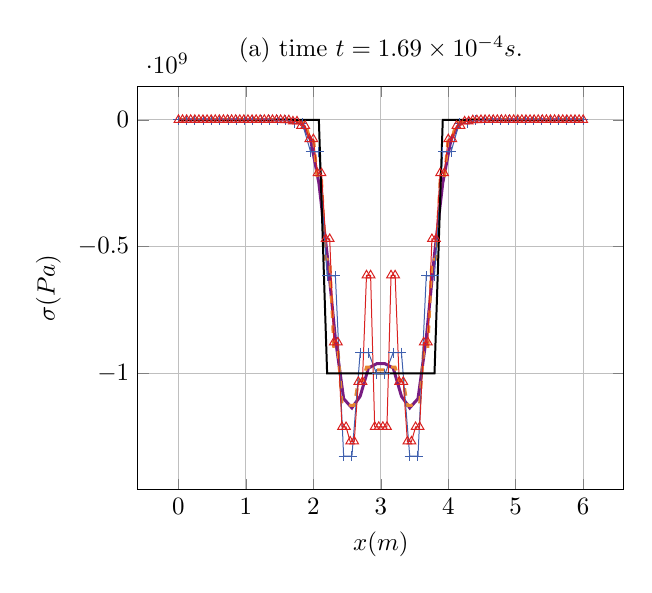
\begin{tikzpicture}[scale=0.9]
\begin{axis}[xlabel=$x (m)$,ylabel=$\sigma (Pa)$,ymajorgrids=true,xmajorgrids=true,title={(a) time $t=1.69 \times 10^{-4} s.$}]
\addplot[Purple,very thick,mark=none,solid] coordinates {(0.0,-9.62200780097e-08) (0.122448979592,-1.92440156019e-07) (0.244897959184,-9.62200780097e-08) (0.367346938776,0.0) (0.489795918367,9.62200780097e-08) (0.612244897959,-9.62200780097e-08) (0.734693877551,-1.92440156019e-07) (0.857142857143,-9.62200780097e-08) (0.979591836735,-9.62200780097e-08) (1.10204081633,0.0) (1.22448979592,9.62200780097e-08) (1.34693877551,-9.62200780097e-08) (1.4693877551,0.0) (1.59183673469,0.0) (1.71428571429,0.0) (1.83673469388,-15437652.4848) (1.95918367347,-78183137.9185) (2.08163265306,-249067223.585) (2.20408163265,-529536815.675) (2.32653061224,-862202048.46) (2.44897959184,-1099498863.41) (2.57142857143,-1135789315.44) (2.69387755102,-1090007223.73) (2.81632653061,-978780358.738) (2.9387755102,-961497360.562) (3.0612244898,-961497360.562) (3.18367346939,-978780358.738) (3.30612244898,-1090007223.73) (3.42857142857,-1135789315.44) (3.55102040816,-1099498863.41) (3.67346938776,-862202048.46) (3.79591836735,-529536815.675) (3.91836734694,-249067223.585) (4.04081632653,-78183137.9185) (4.16326530612,-15437652.4848) (4.28571428571,-3.85185988877e-23) (4.40816326531,-9.62200780097e-08) (4.5306122449,9.62200780097e-08) (4.65306122449,9.62200780097e-08) (4.77551020408,9.62200780097e-08) (4.89795918367,-2.88660234029e-07) (5.02040816327,-9.62200780097e-08) (5.14285714286,9.62200780097e-08) (5.26530612245,1.92440156019e-07) (5.38775510204,2.88660234029e-07) (5.51020408163,9.62200780097e-08) (5.63265306122,0.0) (5.75510204082,0.0) (5.87755102041,0.0) (6.0,-9.62200780097e-08) };
\addplot[Orange,very thick,mark=none,dashed] coordinates {(0.0,0.0) (0.0606060606061,0.0) (0.121212121212,9.52481580298e-08) (0.181818181818,9.52481580298e-08) (0.242424242424,9.52481580298e-08) (0.30303030303,9.52481580298e-08) (0.363636363636,0.0) (0.424242424242,0.0) (0.484848484848,-9.52481580298e-08) (0.545454545455,-9.52481580298e-08) (0.606060606061,-1.9049631606e-07) (0.666666666667,-1.9049631606e-07) (0.727272727273,0.0) (0.787878787879,0.0) (0.848484848485,0.0) (0.909090909091,0.0) (0.969696969697,-3.85185988877e-23) (1.0303030303,-3.85185988877e-23) (1.09090909091,-9.52481580298e-08) (1.15151515152,-9.52481580298e-08) (1.21212121212,9.52481580298e-08) (1.27272727273,9.52481580298e-08) (1.33333333333,9.52481580298e-08) (1.39393939394,9.52481580298e-08) (1.45454545455,-1.9049631606e-07) (1.51515151515,-1.9049631606e-07) (1.57575757576,1.9049631606e-07) (1.63636363636,1.9049631606e-07) (1.69696969697,0.0) (1.75757575758,0.0) (1.81818181818,-9533923.2537) (1.87878787879,-9533923.2537) (1.93939393939,-67166647.336) (2.0,-67166647.336) (2.06060606061,-239339979.822) (2.12121212121,-239339979.822) (2.18181818182,-549695480.518) (2.24242424242,-549695480.518) (2.30303030303,-900240202.504) (2.36363636364,-900240202.504) (2.42424242424,-1118552245.0) (2.48484848485,-1118552245.0) (2.54545454545,-1125362633.2) (2.60606060606,-1125362633.2) (2.66666666667,-1028724363.35) (2.72727272727,-1028724363.35) (2.78787878788,-975375246.836) (2.84848484848,-975375246.836) (2.90909090909,-986009278.185) (2.9696969697,-986009278.185) (3.0303030303,-986009278.185) (3.09090909091,-986009278.185) (3.15151515152,-975375246.836) (3.21212121212,-975375246.836) (3.27272727273,-1028724363.35) (3.33333333333,-1028724363.35) (3.39393939394,-1125362633.2) (3.45454545455,-1125362633.2) (3.51515151515,-1118552245.0) (3.57575757576,-1118552245.0) (3.63636363636,-900240202.504) (3.69696969697,-900240202.504) (3.75757575758,-549695480.518) (3.81818181818,-549695480.518) (3.87878787879,-239339979.822) (3.93939393939,-239339979.822) (4.0,-67166647.336) (4.06060606061,-67166647.336) (4.12121212121,-9533923.2537) (4.18181818182,-9533923.2537) (4.24242424242,9.52481580298e-08) (4.30303030303,9.52481580298e-08) (4.36363636364,-9.52481580298e-08) (4.42424242424,-9.52481580298e-08) (4.48484848485,0.0) (4.54545454545,0.0) (4.60606060606,0.0) (4.66666666667,0.0) (4.72727272727,0.0) (4.78787878788,0.0) (4.84848484848,0.0) (4.90909090909,0.0) (4.9696969697,0.0) (5.0303030303,0.0) (5.09090909091,0.0) (5.15151515152,0.0) (5.21212121212,0.0) (5.27272727273,0.0) (5.33333333333,0.0) (5.39393939394,0.0) (5.45454545455,0.0) (5.51515151515,0.0) (5.57575757576,0.0) (5.63636363636,0.0) (5.69696969697,0.0) (5.75757575758,0.0) (5.81818181818,0.0) (5.87878787879,0.0) (5.93939393939,9.52481580298e-08) (6.0,9.52481580298e-08) };
\addplot[Blue,thin,mark=+,solid] coordinates {(0.0,-3.84880312039e-07) (0.122448979592,2.88660234029e-07) (0.244897959184,-5.77320468058e-07) (0.367346938776,2.88660234029e-07) (0.489795918367,-9.62200780097e-08) (0.612244897959,2.88660234029e-07) (0.734693877551,-4.3483336004) (0.857142857143,-4.34833340796) (0.979591836735,-560.668787915) (1.10204081633,-560.668788299) (1.22448979592,-29850.7439455) (1.34693877551,-29850.7439456) (1.4693877551,-846060.279927) (1.59183673469,-846060.279927) (1.71428571429,-13703737.6015) (1.83673469388,-13703737.6015) (1.95918367347,-126206739.753) (2.08163265306,-126206739.753) (2.20408163265,-614922268.389) (2.32653061224,-614922268.389) (2.44897959184,-1325731906.52) (2.57142857143,-1325731906.52) (2.69387755102,-917663590.795) (2.81632653061,-917663590.795) (2.9387755102,-1001790561.8) (3.0612244898,-1001790561.8) (3.18367346939,-917663590.795) (3.30612244898,-917663590.795) (3.42857142857,-1325731906.52) (3.55102040816,-1325731906.52) (3.67346938776,-614922268.389) (3.79591836735,-614922268.389) (3.91836734694,-126206739.753) (4.04081632653,-126206739.753) (4.16326530612,-13703737.6015) (4.28571428571,-13703737.6015) (4.40816326531,-846060.279927) (4.5306122449,-846060.279927) (4.65306122449,-29850.7439458) (4.77551020408,-29850.7439452) (4.89795918367,-560.668787818) (5.02040816327,-560.668788011) (5.14285714286,-4.34833331174) (5.26530612245,-4.34833340796) (5.38775510204,1.92440156019e-07) (5.51020408163,-9.62200780097e-08) (5.63265306122,1.92440156019e-07) (5.75510204082,-2.88660234029e-07) (5.87755102041,4.81100390048e-07) (6.0,-2.88660234029e-07) };
\addplot[Red,thin,mark=triangle,solid] coordinates {(0.0,0.0) (0.0606060606061,0.0) (0.121212121212,9.52481580298e-08) (0.181818181818,9.52481580298e-08) (0.242424242424,-7.70371977755e-23) (0.30303030303,-7.70371977755e-23) (0.363636363636,-9.52481580298e-08) (0.424242424242,-9.52481580298e-08) (0.484848484848,-1.9049631606e-07) (0.545454545455,-1.9049631606e-07) (0.606060606061,1.9049631606e-07) (0.666666666667,1.9049631606e-07) (0.727272727273,-0.326493160065) (0.787878787879,-0.326493160065) (0.848484848485,-4.24441250957) (0.909090909091,-4.24441250957) (0.969696969697,-75.0667952395) (1.0303030303,-75.0667952395) (1.09090909091,-676.110516968) (1.15151515152,-676.110516968) (1.21212121212,-6409.50756423) (1.27272727273,-6409.50756423) (1.33333333333,-42608.4474487) (1.39393939394,-42608.4474487) (1.45454545455,-271096.202803) (1.51515151515,-271096.202803) (1.57575757576,-1361323.47494) (1.63636363636,-1361323.47494) (1.69696969697,-6186277.73843) (1.75757575758,-6186277.73843) (1.81818181818,-23394049.9045) (1.87878787879,-23394049.9045) (1.93939393939,-76154273.8888) (2.0,-76154273.8888) (2.06060606061,-210327688.316) (2.12121212121,-210327688.316) (2.18181818182,-469773248.386) (2.24242424242,-469773248.386) (2.30303030303,-877374801.132) (2.36363636364,-877374801.132) (2.42424242424,-1211041212.86) (2.48484848485,-1211041212.86) (2.54545454545,-1267995558.57) (2.60606060606,-1267995558.57) (2.66666666667,-1032834595.27) (2.72727272727,-1032834595.27) (2.78787878788,-612908579.142) (2.84848484848,-612908579.142) (2.90909090909,-1210327521.41) (2.9696969697,-1210327521.41) (3.0303030303,-1210327521.41) (3.09090909091,-1210327521.41) (3.15151515152,-612908579.142) (3.21212121212,-612908579.142) (3.27272727273,-1032834595.27) (3.33333333333,-1032834595.27) (3.39393939394,-1267995558.57) (3.45454545455,-1267995558.57) (3.51515151515,-1211041212.86) (3.57575757576,-1211041212.86) (3.63636363636,-877374801.132) (3.69696969697,-877374801.132) (3.75757575758,-469773248.386) (3.81818181818,-469773248.386) (3.87878787879,-210327688.316) (3.93939393939,-210327688.316) (4.0,-76154273.8888) (4.06060606061,-76154273.8888) (4.12121212121,-23394049.9045) (4.18181818182,-23394049.9045) (4.24242424242,-6186277.73843) (4.30303030303,-6186277.73843) (4.36363636364,-1361323.47494) (4.42424242424,-1361323.47494) (4.48484848485,-271096.202803) (4.54545454545,-271096.202803) (4.60606060606,-42608.4474489) (4.66666666667,-42608.4474489) (4.72727272727,-6409.50756433) (4.78787878788,-6409.50756433) (4.84848484848,-676.110516873) (4.90909090909,-676.110516873) (4.9696969697,-75.0667953347) (5.0303030303,-75.0667953347) (5.09090909091,-4.24441231907) (5.15151515152,-4.24441231907) (5.21212121212,-0.326493255313) (5.27272727273,-0.326493255313) (5.33333333333,0.0) (5.39393939394,0.0) (5.45454545455,0.0) (5.51515151515,0.0) (5.57575757576,0.0) (5.63636363636,0.0) (5.69696969697,0.0) (5.75757575758,0.0) (5.81818181818,0.0) (5.87878787879,0.0) (5.93939393939,0.0) (6.0,0.0) };
\addplot[black,thick,mark=none,solid] coordinates {(0.0,-0.0) (0.122448979592,-0.0) (0.244897959184,-0.0) (0.367346938776,-0.0) (0.489795918367,-0.0) (0.612244897959,-0.0) (0.734693877551,-0.0) (0.857142857143,-0.0) (0.979591836735,-0.0) (1.10204081633,-0.0) (1.22448979592,-0.0) (1.34693877551,-0.0) (1.4693877551,-0.0) (1.59183673469,-0.0) (1.71428571429,-0.0) (1.83673469388,-0.0) (1.95918367347,-0.0) (2.08163265306,-0.0) (2.20408163265,-1000000000.0) (2.32653061224,-1000000000.0) (2.44897959184,-1000000000.0) (2.57142857143,-1000000000.0) (2.69387755102,-1000000000.0) (2.81632653061,-1000000000.0) (2.9387755102,-1000000000.0) (3.0612244898,-1000000000.0) (3.18367346939,-1000000000.0) (3.30612244898,-1000000000.0) (3.42857142857,-1000000000.0) (3.55102040816,-1000000000.0) (3.67346938776,-1000000000.0) (3.79591836735,-1000000000.0) (3.91836734694,-0.0) (4.04081632653,-0.0) (4.16326530612,-0.0) (4.28571428571,-0.0) (4.40816326531,-0.0) (4.5306122449,-0.0) (4.65306122449,-0.0) (4.77551020408,-0.0) (4.89795918367,-0.0) (5.02040816327,-0.0) (5.14285714286,-0.0) (5.26530612245,-0.0) (5.38775510204,-0.0) (5.51020408163,-0.0) (5.63265306122,-0.0) (5.75510204082,-0.0) (5.87755102041,-0.0) (6.0,-0.0) };
%\legend{USL 1ppc,USL 2ppc,USF 1ppc,USF 2ppc}
\end{axis}
\end{tikzpicture}
%%% Local Variables:
%%% mode: latex
%%% TeX-master: "../../mainManuscript"
%%% End:
 \phantomsubcaption \label{subfig:US_diffusion_10}}
  {\definecolor{Purple}{RGB}{120,28,129}
\definecolor{Orange}{RGB}{231,133,50}
\definecolor{Blue}{RGB}{63,96,174}
\definecolor{Red}{RGB}{217,33,32}
\definecolor{Duck}{RGB}{83,158,182}
\definecolor{Green}{RGB}{109,179,136}
\definecolor{Yellow}{RGB}{202,184,67}
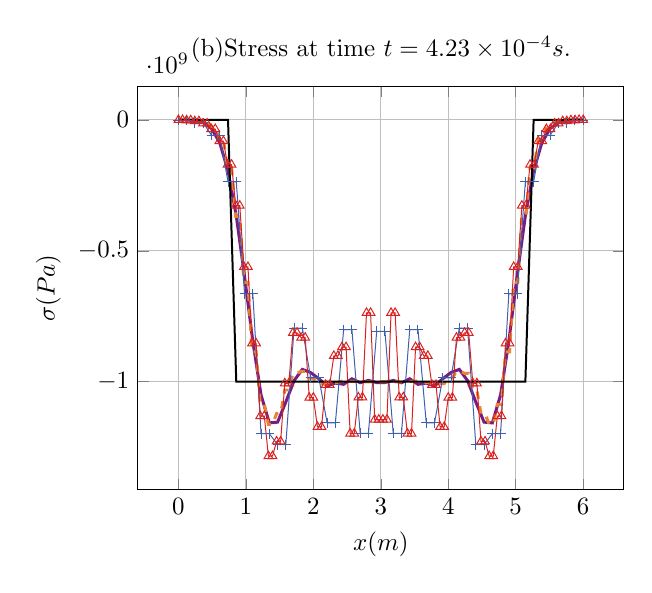
\begin{tikzpicture}[scale=0.9]
\begin{axis}[xlabel=$x (m)$,ylabel=$\sigma (Pa)$,ymajorgrids=true,xmajorgrids=true,title={(b)Stress at time $t= 4.23\times 10^{-4}s.$}]
\addplot[Purple,very thick,mark=none,solid] coordinates {(0.0,-39934.2174897) (0.122448979592,-406302.064953) (0.244897959184,-2420460.88495) (0.367346938776,-10136844.8366) (0.489795918367,-33063216.5915) (0.612244897959,-87547121.3685) (0.734693877551,-194171704.565) (0.857142857143,-366493404.576) (0.979591836735,-596875114.898) (1.10204081633,-845116689.368) (1.22448979592,-1050481005.19) (1.34693877551,-1157297307.0) (1.4693877551,-1154376682.02) (1.59183673469,-1077374033.62) (1.71428571429,-995689036.388) (1.83673469388,-952936697.469) (1.95918367347,-964832377.273) (2.08163265306,-988568067.368) (2.20408163265,-1016260759.09) (2.32653061224,-1005179173.62) (2.44897959184,-1009892551.13) (2.57142857143,-988773783.034) (2.69387755102,-1003829596.99) (2.81632653061,-995025027.704) (2.9387755102,-1003213108.71) (3.0612244898,-1003213108.71) (3.18367346939,-995025027.704) (3.30612244898,-1003829596.99) (3.42857142857,-988773783.034) (3.55102040816,-1009892551.13) (3.67346938776,-1005179173.62) (3.79591836735,-1016260759.09) (3.91836734694,-988568067.368) (4.04081632653,-964832377.273) (4.16326530612,-952936697.469) (4.28571428571,-995689036.388) (4.40816326531,-1077374033.62) (4.5306122449,-1154376682.02) (4.65306122449,-1157297307.0) (4.77551020408,-1050481005.19) (4.89795918367,-845116689.368) (5.02040816327,-596875114.898) (5.14285714286,-366493404.576) (5.26530612245,-194171704.565) (5.38775510204,-87547121.3685) (5.51020408163,-33063216.5915) (5.63265306122,-10136844.8366) (5.75510204082,-2420460.88495) (5.87755102041,-406302.064953) (6.0,-39934.2174897) };
\addplot[Orange,very thick,mark=none,dashed] coordinates {(0.0,-10429.0753611) (0.0606060606061,-10429.0753611) (0.121212121212,-161982.808053) (0.181818181818,-161982.808053) (0.242424242424,-1267409.75703) (0.30303030303,-1267409.75703) (0.363636363636,-6575307.60772) (0.424242424242,-6575307.60772) (0.484848484848,-25213047.7874) (0.545454545455,-25213047.7874) (0.606060606061,-75630068.1866) (0.666666666667,-75630068.1866) (0.727272727273,-183565723.323) (0.787878787879,-183565723.323) (0.848484848485,-368376215.18) (0.909090909091,-368376215.18) (0.969696969697,-620238104.743) (1.0303030303,-620238104.743) (1.09090909091,-886041263.042) (1.15151515152,-886041263.042) (1.21212121212,-1086232263.3) (1.27272727273,-1086232263.3) (1.33333333333,-1162610811.08) (1.39393939394,-1162610811.08) (1.45454545455,-1121800356.23) (1.51515151515,-1121800356.23) (1.57575757576,-1031608883.18) (1.63636363636,-1031608883.18) (1.69696969697,-967968470.151) (1.75757575758,-967968470.151) (1.81818181818,-960540680.349) (1.87878787879,-960540680.349) (1.93939393939,-986227377.719) (2.0,-986227377.719) (2.06060606061,-1007602191.25) (2.12121212121,-1007602191.25) (2.18181818182,-1009726046.8) (2.24242424242,-1009726046.8) (2.30303030303,-1002072997.71) (2.36363636364,-1002072997.71) (2.42424242424,-997465464.463) (2.48484848485,-997465464.463) (2.54545454545,-998318352.653) (2.60606060606,-998318352.653) (2.66666666667,-1000280134.99) (2.72727272727,-1000280134.99) (2.78787878788,-1000550813.71) (2.84848484848,-1000550813.71) (2.90909090909,-999915604.91) (2.9696969697,-999915604.91) (3.0303030303,-999915604.91) (3.09090909091,-999915604.91) (3.15151515152,-1000550813.71) (3.21212121212,-1000550813.71) (3.27272727273,-1000280134.99) (3.33333333333,-1000280134.99) (3.39393939394,-998318352.653) (3.45454545455,-998318352.653) (3.51515151515,-997465464.463) (3.57575757576,-997465464.463) (3.63636363636,-1002072997.71) (3.69696969697,-1002072997.71) (3.75757575758,-1009726046.8) (3.81818181818,-1009726046.8) (3.87878787879,-1007602191.25) (3.93939393939,-1007602191.25) (4.0,-986227377.719) (4.06060606061,-986227377.719) (4.12121212121,-960540680.349) (4.18181818182,-960540680.349) (4.24242424242,-967968470.151) (4.30303030303,-967968470.151) (4.36363636364,-1031608883.18) (4.42424242424,-1031608883.18) (4.48484848485,-1121800356.23) (4.54545454545,-1121800356.23) (4.60606060606,-1162610811.08) (4.66666666667,-1162610811.08) (4.72727272727,-1086232263.3) (4.78787878788,-1086232263.3) (4.84848484848,-886041263.042) (4.90909090909,-886041263.042) (4.9696969697,-620238104.743) (5.0303030303,-620238104.743) (5.09090909091,-368376215.18) (5.15151515152,-368376215.18) (5.21212121212,-183565723.323) (5.27272727273,-183565723.323) (5.33333333333,-75630068.1866) (5.39393939394,-75630068.1866) (5.45454545455,-25213047.7874) (5.51515151515,-25213047.7874) (5.57575757576,-6575307.60772) (5.63636363636,-6575307.60772) (5.69696969697,-1267409.75703) (5.75757575758,-1267409.75703) (5.81818181818,-161982.808054) (5.87878787879,-161982.808054) (5.93939393939,-10429.0753609) (6.0,-10429.0753609) };
\addplot[Blue,thin,mark=+,solid] coordinates {(0.0,-1333876.13913) (0.122448979592,-1333876.13913) (0.244897959184,-10769880.3244) (0.367346938776,-10769880.3244) (0.489795918367,-59004320.4619) (0.612244897959,-59004320.4619) (0.734693877551,-236932522.32) (0.857142857143,-236932522.32) (0.979591836735,-663853517.052) (1.10204081633,-663853517.052) (1.22448979592,-1198320286.6) (1.34693877551,-1198320286.6) (1.4693877551,-1240363116.33) (1.59183673469,-1240363116.33) (1.71428571429,-794840746.96) (1.83673469388,-794840746.96) (1.95918367347,-985342724.542) (2.08163265306,-985342724.542) (2.20408163265,-1157175976.76) (2.32653061224,-1157175976.76) (2.44897959184,-800603512.041) (2.57142857143,-800603512.041) (2.69387755102,-1197082213.94) (2.81632653061,-1197082213.94) (2.9387755102,-808054803.925) (3.0612244898,-808054803.925) (3.18367346939,-1197082213.94) (3.30612244898,-1197082213.94) (3.42857142857,-800603512.041) (3.55102040816,-800603512.041) (3.67346938776,-1157175976.76) (3.79591836735,-1157175976.76) (3.91836734694,-985342724.542) (4.04081632653,-985342724.542) (4.16326530612,-794840746.96) (4.28571428571,-794840746.96) (4.40816326531,-1240363116.33) (4.5306122449,-1240363116.33) (4.65306122449,-1198320286.6) (4.77551020408,-1198320286.6) (4.89795918367,-663853517.052) (5.02040816327,-663853517.052) (5.14285714286,-236932522.32) (5.26530612245,-236932522.32) (5.38775510204,-59004320.4619) (5.51020408163,-59004320.4619) (5.63265306122,-10769880.3244) (5.75510204082,-10769880.3244) (5.87755102041,-1333876.13913) (6.0,-1333876.13913) };
\addplot[Red,thin,mark=triangle] coordinates {(0.0,-388790.247817) (0.0606060606061,-388790.247817) (0.121212121212,-1698682.9889) (0.181818181818,-1698682.9889) (0.242424242424,-5114933.57998) (0.30303030303,-5114933.57998) (0.363636363636,-13968295.6879) (0.424242424242,-13968295.6879) (0.484848484848,-35149039.2515) (0.545454545455,-35149039.2515) (0.606060606061,-81229883.7541) (0.666666666667,-81229883.7541) (0.727272727273,-171384180.27) (0.787878787879,-171384180.27) (0.848484848485,-327574181.976) (0.909090909091,-327574181.976) (0.969696969697,-561694256.942) (1.0303030303,-561694256.942) (1.09090909091,-853480052.942) (1.15151515152,-853480052.942) (1.21212121212,-1131013878.06) (1.27272727273,-1131013878.06) (1.33333333333,-1283904880.31) (1.39393939394,-1283904880.31) (1.45454545455,-1228113384.33) (1.51515151515,-1228113384.33) (1.57575757576,-1005886402.14) (1.63636363636,-1005886402.14) (1.69696969697,-813073422.486) (1.75757575758,-813073422.486) (1.81818181818,-831794248.479) (1.87878787879,-831794248.479) (1.93939393939,-1060904062.7) (2.0,-1060904062.7) (2.06060606061,-1172530924.96) (2.12121212121,-1172530924.96) (2.18181818182,-1012253190.13) (2.24242424242,-1012253190.13) (2.30303030303,-901341875.005) (2.36363636364,-901341875.005) (2.42424242424,-867929277.273) (2.48484848485,-867929277.273) (2.54545454545,-1197799550.43) (2.60606060606,-1197799550.43) (2.66666666667,-1059717228.71) (2.72727272727,-1059717228.71) (2.78787878788,-736963301.649) (2.84848484848,-736963301.649) (2.90909090909,-1144647192.83) (2.9696969697,-1144647192.83) (3.0303030303,-1144647192.83) (3.09090909091,-1144647192.83) (3.15151515152,-736963301.649) (3.21212121212,-736963301.649) (3.27272727273,-1059717228.71) (3.33333333333,-1059717228.71) (3.39393939394,-1197799550.43) (3.45454545455,-1197799550.43) (3.51515151515,-867929277.273) (3.57575757576,-867929277.273) (3.63636363636,-901341875.005) (3.69696969697,-901341875.005) (3.75757575758,-1012253190.13) (3.81818181818,-1012253190.13) (3.87878787879,-1172530924.96) (3.93939393939,-1172530924.96) (4.0,-1060904062.7) (4.06060606061,-1060904062.7) (4.12121212121,-831794248.479) (4.18181818182,-831794248.479) (4.24242424242,-813073422.486) (4.30303030303,-813073422.486) (4.36363636364,-1005886402.14) (4.42424242424,-1005886402.14) (4.48484848485,-1228113384.33) (4.54545454545,-1228113384.33) (4.60606060606,-1283904880.31) (4.66666666667,-1283904880.31) (4.72727272727,-1131013878.06) (4.78787878788,-1131013878.06) (4.84848484848,-853480052.942) (4.90909090909,-853480052.942) (4.9696969697,-561694256.942) (5.0303030303,-561694256.942) (5.09090909091,-327574181.976) (5.15151515152,-327574181.976) (5.21212121212,-171384180.27) (5.27272727273,-171384180.27) (5.33333333333,-81229883.7541) (5.39393939394,-81229883.7541) (5.45454545455,-35149039.2515) (5.51515151515,-35149039.2515) (5.57575757576,-13968295.6879) (5.63636363636,-13968295.6879) (5.69696969697,-5114933.57998) (5.75757575758,-5114933.57998) (5.81818181818,-1698682.9889) (5.87878787879,-1698682.9889) (5.93939393939,-388790.247817) (6.0,-388790.247817) };
\addplot[black,thick] coordinates {(0.0,-0.0) (0.122448979592,-0.0) (0.244897959184,-0.0) (0.367346938776,-0.0) (0.489795918367,-0.0) (0.612244897959,-0.0) (0.734693877551,-0.0) (0.857142857143,-1000000000.0) (0.979591836735,-1000000000.0) (1.10204081633,-1000000000.0) (1.22448979592,-1000000000.0) (1.34693877551,-1000000000.0) (1.4693877551,-1000000000.0) (1.59183673469,-1000000000.0) (1.71428571429,-1000000000.0) (1.83673469388,-1000000000.0) (1.95918367347,-1000000000.0) (2.08163265306,-1000000000.0) (2.20408163265,-1000000000.0) (2.32653061224,-1000000000.0) (2.44897959184,-1000000000.0) (2.57142857143,-1000000000.0) (2.69387755102,-1000000000.0) (2.81632653061,-1000000000.0) (2.9387755102,-1000000000.0) (3.0612244898,-1000000000.0) (3.18367346939,-1000000000.0) (3.30612244898,-1000000000.0) (3.42857142857,-1000000000.0) (3.55102040816,-1000000000.0) (3.67346938776,-1000000000.0) (3.79591836735,-1000000000.0) (3.91836734694,-1000000000.0) (4.04081632653,-1000000000.0) (4.16326530612,-1000000000.0) (4.28571428571,-1000000000.0) (4.40816326531,-1000000000.0) (4.5306122449,-1000000000.0) (4.65306122449,-1000000000.0) (4.77551020408,-1000000000.0) (4.89795918367,-1000000000.0) (5.02040816327,-1000000000.0) (5.14285714286,-1000000000.0) (5.26530612245,-0.0) (5.38775510204,-0.0) (5.51020408163,-0.0) (5.63265306122,-0.0) (5.75510204082,-0.0) (5.87755102041,-0.0) (6.0,-0.0) };
%\legend{USL 1ppc,USL 2ppc,USF 1ppc,USF 2ppc}
\end{axis}
\end{tikzpicture}
%%% Local Variables: 
%%% mode: latex
%%% TeX-master: "../../mainManuscript"
%%% End:
 \phantomsubcaption \label{subfig:US_diffusion_25}}\\
  {\definecolor{Purple}{RGB}{120,28,129}
\definecolor{Orange}{RGB}{231,133,50}
\definecolor{Blue}{RGB}{63,96,174}
\definecolor{Red}{RGB}{217,33,32}
\definecolor{Duck}{RGB}{83,158,182}
\definecolor{Green}{RGB}{109,179,136}
\definecolor{Yellow}{RGB}{202,184,67}
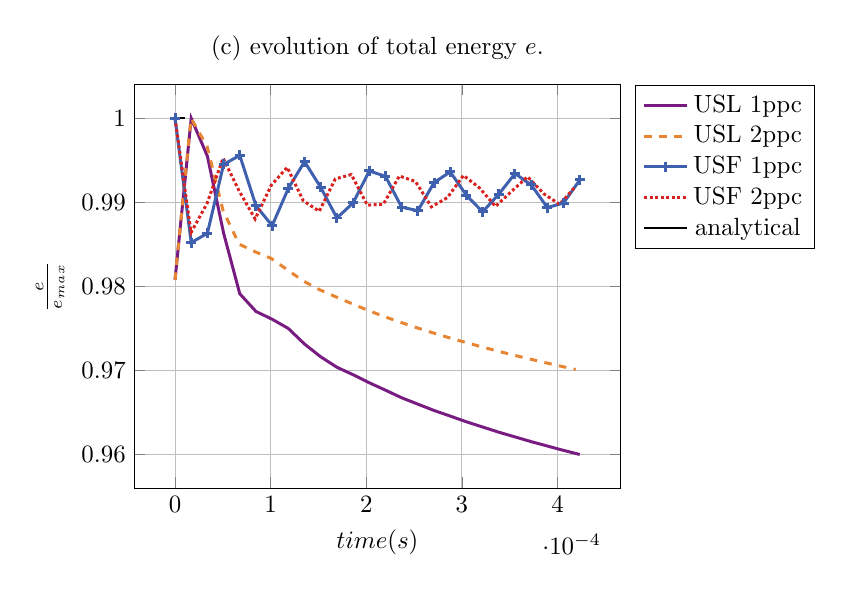
\begin{tikzpicture}[scale=0.9]
\begin{axis}[xlabel=$time (s)$,ylabel=$\frac{e}{e_{max}}$,ymajorgrids=true,xmajorgrids=true,title={(c) evolution of total energy $e$.},legend pos=outer north east]
\addplot[Purple,very thick,mark=none,solid] coordinates {(0.0,0.980776775206) (1.69272151355e-05,1.0) (3.38544302711e-05,0.995486386818) (5.07816454066e-05,0.986335480918) (6.77088605422e-05,0.979118179787) (8.46360756777e-05,0.977011836735) (0.000101563290813,0.976083552705) (0.000118490505949,0.974985958077) (0.000135417721084,0.973132007483) (0.00015234493622,0.971614043952) (0.000169272151355,0.970370597838) (0.000186199366491,0.969484052645) (0.000203126581626,0.968527091175) (0.000220053796762,0.967645365047) (0.000236981011898,0.966743210911) (0.000253908227033,0.965982183586) (0.000270835442169,0.965231974397) (0.000287762657304,0.964563191524) (0.00030468987244,0.96388114719) (0.000321617087575,0.963263530823) (0.000338544302711,0.962646353557) (0.000355471517846,0.962084695394) (0.000372398732982,0.961521764293) (0.000389325948117,0.961001071279) (0.000406253163253,0.960479919884) (0.000423180378389,0.959994795728) };
\addplot[Orange,very thick,mark=none,dashed] coordinates {(0.0,0.980776775206) (1.67562331645e-05,1.0) (3.3512466329e-05,0.996663809337) (5.02686994934e-05,0.98900666995) (6.70249326579e-05,0.985020324447) (8.37811658224e-05,0.984110580813) (0.000100537398987,0.983326915208) (0.000117293632151,0.981979184866) (0.000134049865316,0.980638155666) (0.00015080609848,0.979617302856) (0.000167562331645,0.978778886884) (0.000184318564809,0.977968446843) (0.000201074797974,0.977176694993) (0.000217831031138,0.976440965591) (0.000234587264303,0.975764557777) (0.000251343497467,0.975128766754) (0.000268099730632,0.974522184343) (0.000284855963796,0.973943735564) (0.000301612196961,0.973393220953) (0.000318368430125,0.972867749193) (0.00033512466329,0.972363947434) (0.000351880896454,0.971879647077) (0.000368637129618,0.971413467384) (0.000385393362783,0.970964070517) (0.000402149595947,0.97053007437) (0.000418905829112,0.970110254428) };
\addplot[Blue,very thick,mark=+,solid] coordinates {(0.0,1.0) (1.69272151355e-05,0.985202) (3.38544302711e-05,0.986310925125) (5.07816454066e-05,0.994507638064) (6.77088605422e-05,0.995579868604) (8.46360756777e-05,0.989584575004) (0.000101563290813,0.987225270569) (0.000118490505949,0.991657283729) (0.000135417721084,0.994836102021) (0.00015234493622,0.991773304725) (0.000169272151355,0.988131314159) (0.000186199366491,0.989928559949) (0.000203126581626,0.993725892454) (0.000220053796762,0.993092827557) (0.000236981011898,0.989412077079) (0.000253908227033,0.989007930164) (0.000270835442169,0.992337891088) (0.000287762657304,0.993619763816) (0.00030468987244,0.990831091012) (0.000321617087575,0.988860712515) (0.000338544302711,0.990967493415) (0.000355471517846,0.993415506334) (0.000372398732982,0.99207684926) (0.000389325948117,0.989372657972) (0.000406253163253,0.98991313843) (0.000423180378389,0.992654041387) };
\addplot[Red,very thick,mark=none,densely dotted] coordinates {(0.0,1.0) (1.67562331645e-05,0.9864025) (3.3512466329e-05,0.989873766211) (5.02686994934e-05,0.995255572924) (6.70249326579e-05,0.991355462516) (8.37811658224e-05,0.988011538229) (0.000100537398987,0.992011167376) (0.000117293632151,0.994160481387) (0.000134049865316,0.990189454195) (0.00015080609848,0.988933325063) (0.000167562331645,0.992779930372) (0.000184318564809,0.993300645038) (0.000201074797974,0.989660626012) (0.000217831031138,0.98976821642) (0.000234587264303,0.993129965182) (0.000251343497467,0.992481697852) (0.000268099730632,0.989459518699) (0.000284855963796,0.990567889043) (0.000301612196961,0.993200218105) (0.000318368430125,0.991710475421) (0.00033512466329,0.989506548964) (0.000351880896454,0.99129883371) (0.000368637129618,0.993048080156) (0.000385393362783,0.99103246412) (0.000402149595947,0.989751621209) (0.000418905829112,0.99191164529) };
\addplot[black,thick] coordinates {(0.,1.) (0.00001,1.)};
\legend{USL 1ppc,USL 2ppc,USF 1ppc,USF 2ppc,analytical}
\end{axis}
\end{tikzpicture}
 \phantomsubcaption \label{subfig:US_energies}}
  \caption{MPM solutions of the bars impact problem for various discretizations. (a)--(b) comparison of stress computed with USF and USL formulations and exact solutions (c) numerical total energy evolutions. Parameters: $CFL=0.7$ ; $v_0=\frac{1}{200}\sqrt{\frac{E}{\rho}}$.}
  \label{fig:US_diffusion}
\end{figure}
The stress along the bar at two different time steps (figures \ref{fig:US_diffusion}\subref{subfig:US_diffusion_10} and \ref{fig:US_diffusion}\subref{subfig:US_diffusion_25}) shows that both USL and USF algorithms lead to oscillations around the exact solution regardless of the number of particles per cell. The noise in the MPM solutions is more significant for the USF implementation. On the other, it can be seen in figure \ref{fig:US_diffusion}\subref{subfig:US_energies} that the USL formulation is more diffusive than the USF for this problem. \todo{read \cite{Bardenhagen_USF_USL}} In addition to the previous observations, more significant oscillations appear in the velocity solutions as can be seen in figure \ref{fig:US_velocities} in which the numerical solutions at the last time step of the computation is compared to the exact solution. 
\begin{figure}[h!]
  \centering
  \input{chapter3/pgfFigures/US_velo}
  \caption{Comparison between exact, USF and USL velocities ate the end of the computation of the bars impact problem for various discretizations. Time $t=4.4 \times 10^{-4} \:s.$}
  \label{fig:US_velocities}
\end{figure}


+ Dire un mot sur le HighOrder MPM qui n'est pas forcément désiré car on cherche à approcher des discontinuités.
Dire qu'un champ est défini dans les cellules grâce aux fonctions de forme (notamment dans la forme faible) $q(x)=N_iq_i(x)$, ce qui sous-entend que le mapping inverse doit être fait ainsi.
\begin{figure}[h!]
  \centering
  {\definecolor{Purple}{RGB}{120,28,129}
\definecolor{Orange}{RGB}{231,133,50}
\definecolor{Blue}{RGB}{63,96,174}
\definecolor{Red}{RGB}{217,33,32}
\definecolor{Duck}{RGB}{83,158,182}
\definecolor{Green}{RGB}{109,179,136}
\definecolor{Yellow}{RGB}{202,184,67}
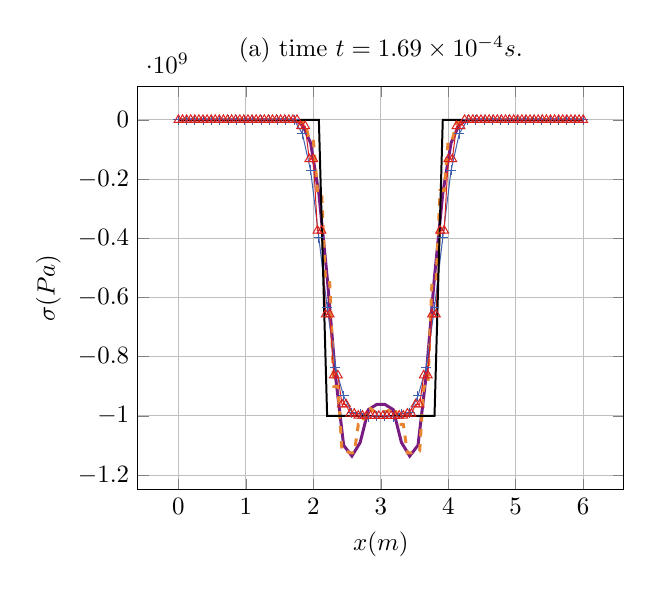
\begin{tikzpicture}[scale=0.9]
\begin{axis}[xlabel=$x (m)$,ylabel=$\sigma (Pa)$,ymajorgrids=true,xmajorgrids=true,title={(a) time $t= 1.69\times 10^{-4}s$.}]
\addplot[Purple,very thick,mark=none,solid] coordinates {(0.0,-9.62200780097e-08) (0.122448979592,-1.92440156019e-07) (0.244897959184,-9.62200780097e-08) (0.367346938776,0.0) (0.489795918367,9.62200780097e-08) (0.612244897959,-9.62200780097e-08) (0.734693877551,-1.92440156019e-07) (0.857142857143,-9.62200780097e-08) (0.979591836735,-9.62200780097e-08) (1.10204081633,0.0) (1.22448979592,9.62200780097e-08) (1.34693877551,-9.62200780097e-08) (1.4693877551,0.0) (1.59183673469,0.0) (1.71428571429,0.0) (1.83673469388,-15437652.4848) (1.95918367347,-78183137.9185) (2.08163265306,-249067223.585) (2.20408163265,-529536815.675) (2.32653061224,-862202048.46) (2.44897959184,-1099498863.41) (2.57142857143,-1135789315.44) (2.69387755102,-1090007223.73) (2.81632653061,-978780358.738) (2.9387755102,-961497360.562) (3.0612244898,-961497360.562) (3.18367346939,-978780358.738) (3.30612244898,-1090007223.73) (3.42857142857,-1135789315.44) (3.55102040816,-1099498863.41) (3.67346938776,-862202048.46) (3.79591836735,-529536815.675) (3.91836734694,-249067223.585) (4.04081632653,-78183137.9185) (4.16326530612,-15437652.4848) (4.28571428571,-3.85185988877e-23) (4.40816326531,-9.62200780097e-08) (4.5306122449,9.62200780097e-08) (4.65306122449,9.62200780097e-08) (4.77551020408,9.62200780097e-08) (4.89795918367,-2.88660234029e-07) (5.02040816327,-9.62200780097e-08) (5.14285714286,9.62200780097e-08) (5.26530612245,1.92440156019e-07) (5.38775510204,2.88660234029e-07) (5.51020408163,9.62200780097e-08) (5.63265306122,0.0) (5.75510204082,0.0) (5.87755102041,0.0) (6.0,-9.62200780097e-08) };
\addplot[Orange,very thick,mark=none,dashed] coordinates {(0.0,0.0) (0.0606060606061,0.0) (0.121212121212,9.52481580298e-08) (0.181818181818,9.52481580298e-08) (0.242424242424,9.52481580298e-08) (0.30303030303,9.52481580298e-08) (0.363636363636,0.0) (0.424242424242,0.0) (0.484848484848,-9.52481580298e-08) (0.545454545455,-9.52481580298e-08) (0.606060606061,-1.9049631606e-07) (0.666666666667,-1.9049631606e-07) (0.727272727273,0.0) (0.787878787879,0.0) (0.848484848485,0.0) (0.909090909091,0.0) (0.969696969697,-3.85185988877e-23) (1.0303030303,-3.85185988877e-23) (1.09090909091,-9.52481580298e-08) (1.15151515152,-9.52481580298e-08) (1.21212121212,9.52481580298e-08) (1.27272727273,9.52481580298e-08) (1.33333333333,9.52481580298e-08) (1.39393939394,9.52481580298e-08) (1.45454545455,-1.9049631606e-07) (1.51515151515,-1.9049631606e-07) (1.57575757576,1.9049631606e-07) (1.63636363636,1.9049631606e-07) (1.69696969697,0.0) (1.75757575758,0.0) (1.81818181818,-9533923.2537) (1.87878787879,-9533923.2537) (1.93939393939,-67166647.336) (2.0,-67166647.336) (2.06060606061,-239339979.822) (2.12121212121,-239339979.822) (2.18181818182,-549695480.518) (2.24242424242,-549695480.518) (2.30303030303,-900240202.504) (2.36363636364,-900240202.504) (2.42424242424,-1118552245.0) (2.48484848485,-1118552245.0) (2.54545454545,-1125362633.2) (2.60606060606,-1125362633.2) (2.66666666667,-1028724363.35) (2.72727272727,-1028724363.35) (2.78787878788,-975375246.836) (2.84848484848,-975375246.836) (2.90909090909,-986009278.185) (2.9696969697,-986009278.185) (3.0303030303,-986009278.185) (3.09090909091,-986009278.185) (3.15151515152,-975375246.836) (3.21212121212,-975375246.836) (3.27272727273,-1028724363.35) (3.33333333333,-1028724363.35) (3.39393939394,-1125362633.2) (3.45454545455,-1125362633.2) (3.51515151515,-1118552245.0) (3.57575757576,-1118552245.0) (3.63636363636,-900240202.504) (3.69696969697,-900240202.504) (3.75757575758,-549695480.518) (3.81818181818,-549695480.518) (3.87878787879,-239339979.822) (3.93939393939,-239339979.822) (4.0,-67166647.336) (4.06060606061,-67166647.336) (4.12121212121,-9533923.2537) (4.18181818182,-9533923.2537) (4.24242424242,9.52481580298e-08) (4.30303030303,9.52481580298e-08) (4.36363636364,-9.52481580298e-08) (4.42424242424,-9.52481580298e-08) (4.48484848485,0.0) (4.54545454545,0.0) (4.60606060606,0.0) (4.66666666667,0.0) (4.72727272727,0.0) (4.78787878788,0.0) (4.84848484848,0.0) (4.90909090909,0.0) (4.9696969697,0.0) (5.0303030303,0.0) (5.09090909091,0.0) (5.15151515152,0.0) (5.21212121212,0.0) (5.27272727273,0.0) (5.33333333333,0.0) (5.39393939394,0.0) (5.45454545455,0.0) (5.51515151515,0.0) (5.57575757576,0.0) (5.63636363636,0.0) (5.69696969697,0.0) (5.75757575758,0.0) (5.81818181818,0.0) (5.87878787879,0.0) (5.93939393939,9.52481580298e-08) (6.0,9.52481580298e-08) };
\addplot[Blue,thin,mark=+,solid] coordinates {(0.0,9.62200780097e-08) (0.122448979592,1.92440156019e-07) (0.244897959184,-2.88660234029e-07) (0.367346938776,-1.92440156019e-07) (0.489795918367,-9.62200780097e-08) (0.612244897959,-1.92440156019e-07) (0.734693877551,-3.84880312039e-07) (0.857142857143,-1.92440156019e-07) (0.979591836735,-9.62200780097e-08) (1.10204081633,0.0) (1.22448979592,9.62200780097e-08) (1.34693877551,-9.62200780097e-08) (1.4693877551,0.0) (1.59183673469,0.0) (1.71428571429,0.0) (1.83673469388,-46578287.5426) (1.95918367347,-171036560.611) (2.08163265306,-398499931.778) (2.20408163265,-632823078.817) (2.32653061224,-835128021.529) (2.44897959184,-932849760.398) (2.57142857143,-988852888.782) (2.69387755102,-992828858.011) (2.81632653061,-1002356300.0) (2.9387755102,-999046312.534) (3.0612244898,-999046312.534) (3.18367346939,-1002356300.0) (3.30612244898,-992828858.011) (3.42857142857,-988852888.782) (3.55102040816,-932849760.398) (3.67346938776,-835128021.529) (3.79591836735,-632823078.817) (3.91836734694,-398499931.778) (4.04081632653,-171036560.611) (4.16326530612,-46578287.5426) (4.28571428571,0.0) (4.40816326531,-9.62200780097e-08) (4.5306122449,-1.92592994439e-23) (4.65306122449,1.92440156019e-07) (4.77551020408,0.0) (4.89795918367,-9.62200780097e-08) (5.02040816327,0.0) (5.14285714286,0.0) (5.26530612245,3.85185988877e-23) (5.38775510204,1.92440156019e-07) (5.51020408163,9.62200780097e-08) (5.63265306122,0.0) (5.75510204082,9.62200780097e-08) (5.87755102041,0.0) (6.0,-9.62200780097e-08) };
\addplot[Red,thin,mark=triangle,solid] coordinates {(0.0,-1.9049631606e-07) (0.0606060606061,-1.9049631606e-07) (0.121212121212,0.0) (0.181818181818,0.0) (0.242424242424,9.52481580298e-08) (0.30303030303,9.52481580298e-08) (0.363636363636,-9.52481580298e-08) (0.424242424242,-9.52481580298e-08) (0.484848484848,-1.9049631606e-07) (0.545454545455,-1.9049631606e-07) (0.606060606061,0.0) (0.666666666667,0.0) (0.727272727273,0.0) (0.787878787879,0.0) (0.848484848485,0.0) (0.909090909091,0.0) (0.969696969697,-9.52481580298e-08) (1.0303030303,-9.52481580298e-08) (1.09090909091,-1.9049631606e-07) (1.15151515152,-1.9049631606e-07) (1.21212121212,-9.52481580298e-08) (1.27272727273,-9.52481580298e-08) (1.33333333333,0.0) (1.39393939394,0.0) (1.45454545455,9.52481580298e-08) (1.51515151515,9.52481580298e-08) (1.57575757576,-9.52481580298e-08) (1.63636363636,-9.52481580298e-08) (1.69696969697,0.0) (1.75757575758,0.0) (1.81818181818,-21051436.477) (1.87878787879,-21051436.477) (1.93939393939,-132631129.917) (2.0,-132631129.917) (2.06060606061,-373920143.932) (2.12121212121,-373920143.932) (2.18181818182,-657449507.004) (2.24242424242,-657449507.004) (2.30303030303,-862932918.65) (2.36363636364,-862932918.65) (2.42424242424,-960874193.44) (2.48484848485,-960874193.44) (2.54545454545,-992227161.455) (2.60606060606,-992227161.455) (2.66666666667,-998999192.727) (2.72727272727,-998999192.727) (2.78787878788,-999914743.293) (2.84848484848,-999914743.293) (2.90909090909,-999999573.105) (2.9696969697,-999999573.105) (3.0303030303,-999999573.105) (3.09090909091,-999999573.105) (3.15151515152,-999914743.293) (3.21212121212,-999914743.293) (3.27272727273,-998999192.727) (3.33333333333,-998999192.727) (3.39393939394,-992227161.455) (3.45454545455,-992227161.455) (3.51515151515,-960874193.44) (3.57575757576,-960874193.44) (3.63636363636,-862932918.65) (3.69696969697,-862932918.65) (3.75757575758,-657449507.004) (3.81818181818,-657449507.004) (3.87878787879,-373920143.932) (3.93939393939,-373920143.932) (4.0,-132631129.917) (4.06060606061,-132631129.917) (4.12121212121,-21051436.477) (4.18181818182,-21051436.477) (4.24242424242,-9.52481580298e-08) (4.30303030303,-9.52481580298e-08) (4.36363636364,9.52481580298e-08) (4.42424242424,9.52481580298e-08) (4.48484848485,0.0) (4.54545454545,0.0) (4.60606060606,0.0) (4.66666666667,0.0) (4.72727272727,0.0) (4.78787878788,0.0) (4.84848484848,0.0) (4.90909090909,0.0) (4.9696969697,0.0) (5.0303030303,0.0) (5.09090909091,0.0) (5.15151515152,0.0) (5.21212121212,0.0) (5.27272727273,0.0) (5.33333333333,0.0) (5.39393939394,0.0) (5.45454545455,0.0) (5.51515151515,0.0) (5.57575757576,0.0) (5.63636363636,0.0) (5.69696969697,0.0) (5.75757575758,0.0) (5.81818181818,0.0) (5.87878787879,0.0) (5.93939393939,-1.9049631606e-07) (6.0,-1.9049631606e-07) };
\addplot[black,thick,mark=none,solid] coordinates {(0.0,-0.0) (0.122448979592,-0.0) (0.244897959184,-0.0) (0.367346938776,-0.0) (0.489795918367,-0.0) (0.612244897959,-0.0) (0.734693877551,-0.0) (0.857142857143,-0.0) (0.979591836735,-0.0) (1.10204081633,-0.0) (1.22448979592,-0.0) (1.34693877551,-0.0) (1.4693877551,-0.0) (1.59183673469,-0.0) (1.71428571429,-0.0) (1.83673469388,-0.0) (1.95918367347,-0.0) (2.08163265306,-0.0) (2.20408163265,-1000000000.0) (2.32653061224,-1000000000.0) (2.44897959184,-1000000000.0) (2.57142857143,-1000000000.0) (2.69387755102,-1000000000.0) (2.81632653061,-1000000000.0) (2.9387755102,-1000000000.0) (3.0612244898,-1000000000.0) (3.18367346939,-1000000000.0) (3.30612244898,-1000000000.0) (3.42857142857,-1000000000.0) (3.55102040816,-1000000000.0) (3.67346938776,-1000000000.0) (3.79591836735,-1000000000.0) (3.91836734694,-0.0) (4.04081632653,-0.0) (4.16326530612,-0.0) (4.28571428571,-0.0) (4.40816326531,-0.0) (4.5306122449,-0.0) (4.65306122449,-0.0) (4.77551020408,-0.0) (4.89795918367,-0.0) (5.02040816327,-0.0) (5.14285714286,-0.0) (5.26530612245,-0.0) (5.38775510204,-0.0) (5.51020408163,-0.0) (5.63265306122,-0.0) (5.75510204082,-0.0) (5.87755102041,-0.0) (6.0,-0.0) };
%\legend{MPM 1ppc,MPM 2ppc,Mod.Map. 1ppc,Mod.Map. 2ppc,analytic}
\end{axis}
\end{tikzpicture}
 \phantomsubcaption \label{subfig:mpm_diffusion_10}}
  {\definecolor{Purple}{RGB}{120,28,129}
\definecolor{Orange}{RGB}{231,133,50}
\definecolor{Blue}{RGB}{63,96,174}
\definecolor{Red}{RGB}{217,33,32}
\definecolor{Duck}{RGB}{83,158,182}
\definecolor{Green}{RGB}{109,179,136}
\definecolor{Yellow}{RGB}{202,184,67}
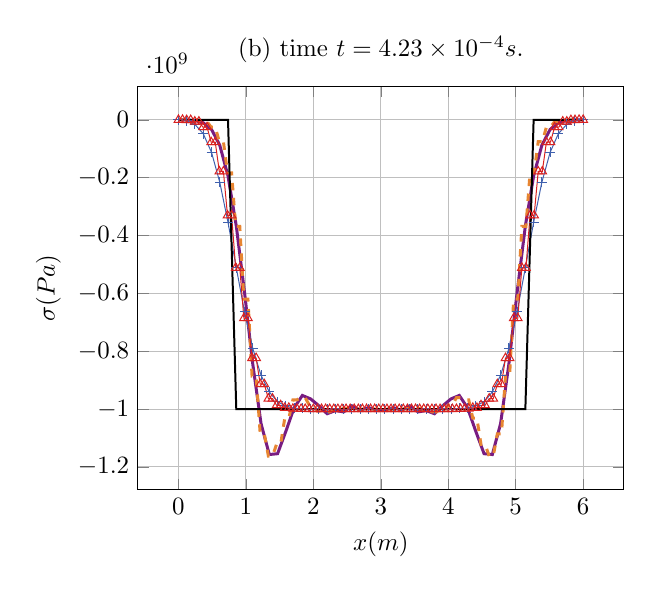
\begin{tikzpicture}[scale=0.9]
\begin{axis}[xlabel=$x (m)$,ylabel=$\sigma (Pa)$,ymajorgrids=true,xmajorgrids=true,title={(b) time $t= 4.23\times 10^{-4}s$.}]
\addplot[Purple,very thick,mark=none,solid] coordinates {(0.0,-39934.2174897) (0.122448979592,-406302.064953) (0.244897959184,-2420460.88495) (0.367346938776,-10136844.8366) (0.489795918367,-33063216.5915) (0.612244897959,-87547121.3685) (0.734693877551,-194171704.565) (0.857142857143,-366493404.576) (0.979591836735,-596875114.898) (1.10204081633,-845116689.368) (1.22448979592,-1050481005.19) (1.34693877551,-1157297307.0) (1.4693877551,-1154376682.02) (1.59183673469,-1077374033.62) (1.71428571429,-995689036.388) (1.83673469388,-952936697.469) (1.95918367347,-964832377.273) (2.08163265306,-988568067.368) (2.20408163265,-1016260759.09) (2.32653061224,-1005179173.62) (2.44897959184,-1009892551.13) (2.57142857143,-988773783.034) (2.69387755102,-1003829596.99) (2.81632653061,-995025027.704) (2.9387755102,-1003213108.71) (3.0612244898,-1003213108.71) (3.18367346939,-995025027.704) (3.30612244898,-1003829596.99) (3.42857142857,-988773783.034) (3.55102040816,-1009892551.13) (3.67346938776,-1005179173.62) (3.79591836735,-1016260759.09) (3.91836734694,-988568067.368) (4.04081632653,-964832377.273) (4.16326530612,-952936697.469) (4.28571428571,-995689036.388) (4.40816326531,-1077374033.62) (4.5306122449,-1154376682.02) (4.65306122449,-1157297307.0) (4.77551020408,-1050481005.19) (4.89795918367,-845116689.368) (5.02040816327,-596875114.898) (5.14285714286,-366493404.576) (5.26530612245,-194171704.565) (5.38775510204,-87547121.3685) (5.51020408163,-33063216.5915) (5.63265306122,-10136844.8366) (5.75510204082,-2420460.88495) (5.87755102041,-406302.064953) (6.0,-39934.2174897) };
\addplot[Orange,very thick,mark=none,dashed] coordinates {(0.0,-10429.0753611) (0.0606060606061,-10429.0753611) (0.121212121212,-161982.808053) (0.181818181818,-161982.808053) (0.242424242424,-1267409.75703) (0.30303030303,-1267409.75703) (0.363636363636,-6575307.60772) (0.424242424242,-6575307.60772) (0.484848484848,-25213047.7874) (0.545454545455,-25213047.7874) (0.606060606061,-75630068.1866) (0.666666666667,-75630068.1866) (0.727272727273,-183565723.323) (0.787878787879,-183565723.323) (0.848484848485,-368376215.18) (0.909090909091,-368376215.18) (0.969696969697,-620238104.743) (1.0303030303,-620238104.743) (1.09090909091,-886041263.042) (1.15151515152,-886041263.042) (1.21212121212,-1086232263.3) (1.27272727273,-1086232263.3) (1.33333333333,-1162610811.08) (1.39393939394,-1162610811.08) (1.45454545455,-1121800356.23) (1.51515151515,-1121800356.23) (1.57575757576,-1031608883.18) (1.63636363636,-1031608883.18) (1.69696969697,-967968470.151) (1.75757575758,-967968470.151) (1.81818181818,-960540680.349) (1.87878787879,-960540680.349) (1.93939393939,-986227377.719) (2.0,-986227377.719) (2.06060606061,-1007602191.25) (2.12121212121,-1007602191.25) (2.18181818182,-1009726046.8) (2.24242424242,-1009726046.8) (2.30303030303,-1002072997.71) (2.36363636364,-1002072997.71) (2.42424242424,-997465464.463) (2.48484848485,-997465464.463) (2.54545454545,-998318352.653) (2.60606060606,-998318352.653) (2.66666666667,-1000280134.99) (2.72727272727,-1000280134.99) (2.78787878788,-1000550813.71) (2.84848484848,-1000550813.71) (2.90909090909,-999915604.91) (2.9696969697,-999915604.91) (3.0303030303,-999915604.91) (3.09090909091,-999915604.91) (3.15151515152,-1000550813.71) (3.21212121212,-1000550813.71) (3.27272727273,-1000280134.99) (3.33333333333,-1000280134.99) (3.39393939394,-998318352.653) (3.45454545455,-998318352.653) (3.51515151515,-997465464.463) (3.57575757576,-997465464.463) (3.63636363636,-1002072997.71) (3.69696969697,-1002072997.71) (3.75757575758,-1009726046.8) (3.81818181818,-1009726046.8) (3.87878787879,-1007602191.25) (3.93939393939,-1007602191.25) (4.0,-986227377.719) (4.06060606061,-986227377.719) (4.12121212121,-960540680.349) (4.18181818182,-960540680.349) (4.24242424242,-967968470.151) (4.30303030303,-967968470.151) (4.36363636364,-1031608883.18) (4.42424242424,-1031608883.18) (4.48484848485,-1121800356.23) (4.54545454545,-1121800356.23) (4.60606060606,-1162610811.08) (4.66666666667,-1162610811.08) (4.72727272727,-1086232263.3) (4.78787878788,-1086232263.3) (4.84848484848,-886041263.042) (4.90909090909,-886041263.042) (4.9696969697,-620238104.743) (5.0303030303,-620238104.743) (5.09090909091,-368376215.18) (5.15151515152,-368376215.18) (5.21212121212,-183565723.323) (5.27272727273,-183565723.323) (5.33333333333,-75630068.1866) (5.39393939394,-75630068.1866) (5.45454545455,-25213047.7874) (5.51515151515,-25213047.7874) (5.57575757576,-6575307.60772) (5.63636363636,-6575307.60772) (5.69696969697,-1267409.75703) (5.75757575758,-1267409.75703) (5.81818181818,-161982.808054) (5.87878787879,-161982.808054) (5.93939393939,-10429.0753609) (6.0,-10429.0753609) };
\addplot[Blue,thin,mark=+,solid] coordinates {(0.0,-508931.478279) (0.122448979592,-3748025.68591) (0.244897959184,-16014385.4746) (0.367346938776,-47881742.3505) (0.489795918367,-112174746.169) (0.612244897959,-215592738.441) (0.734693877551,-354671855.848) (0.857142857143,-511212799.02) (0.979591836735,-663838312.129) (1.10204081633,-790213464.162) (1.22448979592,-883647482.448) (1.34693877551,-941000619.105) (1.4693877551,-974959939.111) (1.59183673469,-988927861.484) (1.71428571429,-997557909.852) (1.83673469388,-997805889.972) (1.95918367347,-1000931915.66) (2.08163265306,-998709339.041) (2.20408163265,-1001197182.01) (2.32653061224,-998859728.815) (2.44897959184,-1001017871.89) (2.57142857143,-999150004.014) (2.69387755102,-1000640138.33) (2.81632653061,-999602146.851) (2.9387755102,-1000134970.66) (3.0612244898,-1000134970.66) (3.18367346939,-999602146.851) (3.30612244898,-1000640138.33) (3.42857142857,-999150004.014) (3.55102040816,-1001017871.89) (3.67346938776,-998859728.815) (3.79591836735,-1001197182.01) (3.91836734694,-998709339.041) (4.04081632653,-1000931915.66) (4.16326530612,-997805889.972) (4.28571428571,-997557909.852) (4.40816326531,-988927861.484) (4.5306122449,-974959939.111) (4.65306122449,-941000619.105) (4.77551020408,-883647482.448) (4.89795918367,-790213464.162) (5.02040816327,-663838312.129) (5.14285714286,-511212799.02) (5.26530612245,-354671855.848) (5.38775510204,-215592738.441) (5.51020408163,-112174746.169) (5.63265306122,-47881742.3505) (5.75510204082,-16014385.4746) (5.87755102041,-3748025.68591) (6.0,-508931.478279) };
\addplot[Red,thin,mark=triangle,solid] coordinates {(0.0,-61223.9335744) (0.0606060606061,-61223.9335744) (0.121212121212,-884894.710625) (0.181818181818,-884894.710625) (0.242424242424,-6003361.51961) (0.30303030303,-6003361.51961) (0.363636363636,-25575128.3809) (0.424242424242,-25575128.3809) (0.484848484848,-77365275.2782) (0.545454545455,-77365275.2782) (0.606060606061,-178548645.631) (0.666666666667,-178548645.631) (0.727272727273,-330659471.659) (0.787878787879,-330659471.659) (0.848484848485,-511731335.491) (0.909090909091,-511731335.491) (0.969696969697,-686005012.829) (1.0303030303,-686005012.829) (1.09090909091,-823733433.992) (1.15151515152,-823733433.992) (1.21212121212,-914145742.521) (1.27272727273,-914145742.521) (1.33333333333,-963861687.734) (1.39393939394,-963861687.734) (1.45454545455,-986895334.229) (1.51515151515,-986895334.229) (1.57575757576,-995919063.725) (1.63636363636,-995919063.725) (1.69696969697,-998912836.991) (1.75757575758,-998912836.991) (1.81818181818,-999753499.27) (1.87878787879,-999753499.27) (1.93939393939,-999952757.55) (2.0,-999952757.55) (2.06060606061,-999992418.488) (2.12121212121,-999992418.488) (2.18181818182,-999998994.239) (2.24242424242,-999998994.239) (2.30303030303,-999999891.711) (2.36363636364,-999999891.711) (2.42424242424,-999999990.727) (2.48484848485,-999999990.727) (2.54545454545,-999999999.438) (2.60606060606,-999999999.438) (2.66666666667,-999999999.942) (2.72727272727,-999999999.942) (2.78787878788,-1000000000.02) (2.84848484848,-1000000000.02) (2.90909090909,-999999999.993) (2.9696969697,-999999999.993) (3.0303030303,-999999999.993) (3.09090909091,-999999999.993) (3.15151515152,-1000000000.02) (3.21212121212,-1000000000.02) (3.27272727273,-999999999.942) (3.33333333333,-999999999.942) (3.39393939394,-999999999.438) (3.45454545455,-999999999.438) (3.51515151515,-999999990.727) (3.57575757576,-999999990.727) (3.63636363636,-999999891.711) (3.69696969697,-999999891.711) (3.75757575758,-999998994.239) (3.81818181818,-999998994.239) (3.87878787879,-999992418.488) (3.93939393939,-999992418.488) (4.0,-999952757.55) (4.06060606061,-999952757.55) (4.12121212121,-999753499.27) (4.18181818182,-999753499.27) (4.24242424242,-998912836.991) (4.30303030303,-998912836.991) (4.36363636364,-995919063.725) (4.42424242424,-995919063.725) (4.48484848485,-986895334.229) (4.54545454545,-986895334.229) (4.60606060606,-963861687.734) (4.66666666667,-963861687.734) (4.72727272727,-914145742.521) (4.78787878788,-914145742.521) (4.84848484848,-823733433.992) (4.90909090909,-823733433.992) (4.9696969697,-686005012.829) (5.0303030303,-686005012.829) (5.09090909091,-511731335.491) (5.15151515152,-511731335.491) (5.21212121212,-330659471.659) (5.27272727273,-330659471.659) (5.33333333333,-178548645.631) (5.39393939394,-178548645.631) (5.45454545455,-77365275.2782) (5.51515151515,-77365275.2782) (5.57575757576,-25575128.3809) (5.63636363636,-25575128.3809) (5.69696969697,-6003361.51961) (5.75757575758,-6003361.51961) (5.81818181818,-884894.710625) (5.87878787879,-884894.710625) (5.93939393939,-61223.9335744) (6.0,-61223.9335744) };
\addplot[black,thick,mark=none,solid] coordinates {(0.0,-0.0) (0.122448979592,-0.0) (0.244897959184,-0.0) (0.367346938776,-0.0) (0.489795918367,-0.0) (0.612244897959,-0.0) (0.734693877551,-0.0) (0.857142857143,-1000000000.0) (0.979591836735,-1000000000.0) (1.10204081633,-1000000000.0) (1.22448979592,-1000000000.0) (1.34693877551,-1000000000.0) (1.4693877551,-1000000000.0) (1.59183673469,-1000000000.0) (1.71428571429,-1000000000.0) (1.83673469388,-1000000000.0) (1.95918367347,-1000000000.0) (2.08163265306,-1000000000.0) (2.20408163265,-1000000000.0) (2.32653061224,-1000000000.0) (2.44897959184,-1000000000.0) (2.57142857143,-1000000000.0) (2.69387755102,-1000000000.0) (2.81632653061,-1000000000.0) (2.9387755102,-1000000000.0) (3.0612244898,-1000000000.0) (3.18367346939,-1000000000.0) (3.30612244898,-1000000000.0) (3.42857142857,-1000000000.0) (3.55102040816,-1000000000.0) (3.67346938776,-1000000000.0) (3.79591836735,-1000000000.0) (3.91836734694,-1000000000.0) (4.04081632653,-1000000000.0) (4.16326530612,-1000000000.0) (4.28571428571,-1000000000.0) (4.40816326531,-1000000000.0) (4.5306122449,-1000000000.0) (4.65306122449,-1000000000.0) (4.77551020408,-1000000000.0) (4.89795918367,-1000000000.0) (5.02040816327,-1000000000.0) (5.14285714286,-1000000000.0) (5.26530612245,-0.0) (5.38775510204,-0.0) (5.51020408163,-0.0) (5.63265306122,-0.0) (5.75510204082,-0.0) (5.87755102041,-0.0) (6.0,-0.0) };
%\legend{MPM 1ppc,MPM 2ppc,Mod.Map. 1ppc,Mod.Map. 2ppc,analytic}
\end{axis}
\end{tikzpicture}
 \phantomsubcaption \label{subfig:mpm_diffusion_25}}\\
  {\definecolor{Purple}{RGB}{120,28,129}
\definecolor{Orange}{RGB}{231,133,50}
\definecolor{Blue}{RGB}{63,96,174}
\definecolor{Red}{RGB}{217,33,32}
\definecolor{Duck}{RGB}{83,158,182}
\definecolor{Green}{RGB}{109,179,136}
\definecolor{Yellow}{RGB}{202,184,67}
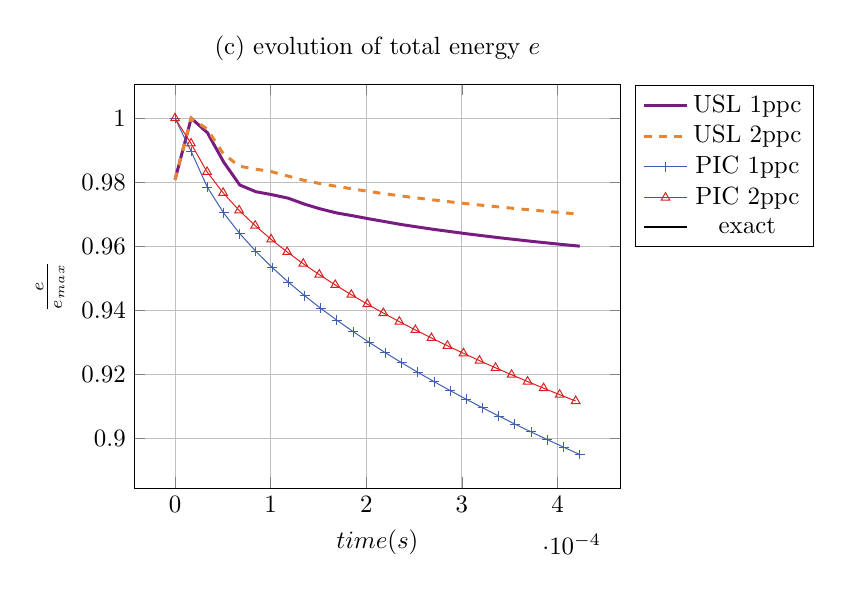
\begin{tikzpicture}[scale=0.9]
\begin{axis}[xlabel=$time (s)$,ylabel=$\frac{e}{e_{max}}$,ymajorgrids=true,xmajorgrids=true,title={(c) evolution of total energy $e$},legend pos=outer north east]
\addplot[Purple,very thick,mark=none,solid] coordinates {(0.0,0.980776775206) (1.69272151355e-05,1.0) (3.38544302711e-05,0.995486386818) (5.07816454066e-05,0.986335480918) (6.77088605422e-05,0.979118179787) (8.46360756777e-05,0.977011836735) (0.000101563290813,0.976083552705) (0.000118490505949,0.974985958077) (0.000135417721084,0.973132007483) (0.00015234493622,0.971614043952) (0.000169272151355,0.970370597838) (0.000186199366491,0.969484052645) (0.000203126581626,0.968527091175) (0.000220053796762,0.967645365047) (0.000236981011898,0.966743210911) (0.000253908227033,0.965982183586) (0.000270835442169,0.965231974397) (0.000287762657304,0.964563191524) (0.00030468987244,0.96388114719) (0.000321617087575,0.963263530823) (0.000338544302711,0.962646353557) (0.000355471517846,0.962084695394) (0.000372398732982,0.961521764293) (0.000389325948117,0.961001071279) (0.000406253163253,0.960479919884) (0.000423180378389,0.959994795728) };
\addplot[Orange,very thick,mark=none,dashed] coordinates {(0.0,0.980776775206) (1.67562331645e-05,1.0) (3.3512466329e-05,0.996663809337) (5.02686994934e-05,0.98900666995) (6.70249326579e-05,0.985020324447) (8.37811658224e-05,0.984110580813) (0.000100537398987,0.983326915208) (0.000117293632151,0.981979184866) (0.000134049865316,0.980638155666) (0.00015080609848,0.979617302856) (0.000167562331645,0.978778886884) (0.000184318564809,0.977968446843) (0.000201074797974,0.977176694993) (0.000217831031138,0.976440965591) (0.000234587264303,0.975764557777) (0.000251343497467,0.975128766754) (0.000268099730632,0.974522184343) (0.000284855963796,0.973943735564) (0.000301612196961,0.973393220953) (0.000318368430125,0.972867749193) (0.00033512466329,0.972363947434) (0.000351880896454,0.971879647077) (0.000368637129618,0.971413467384) (0.000385393362783,0.970964070517) (0.000402149595947,0.97053007437) (0.000418905829112,0.970110254428) };
\addplot[Blue,thin,mark=+,solid] coordinates {(0.0,1.0) (1.69272151355e-05,0.9896) (3.38544302711e-05,0.97840192) (5.07816454066e-05,0.970395814144) (6.77088605422e-05,0.963922377931) (8.46360756777e-05,0.958330092512) (0.000101563290813,0.953327939993) (0.000118490505949,0.948758714644) (0.000135417721084,0.944525461648) (0.00015234493622,0.940563061208) (0.000169272151355,0.936825160363) (0.000186199366491,0.933277336034) (0.000203126581626,0.929893178182) (0.000220053796762,0.926651891851) (0.000236981011898,0.923536752237) (0.000253908227033,0.92053406787) (0.000270835442169,0.917632461061) (0.000287762657304,0.914822354268) (0.00030468987244,0.912095594541) (0.000321617087575,0.909445173164) (0.000338544302711,0.906865012545) (0.000355471517846,0.904349801607) (0.000372398732982,0.901894866831) (0.000389325948117,0.899496069935) (0.000406253163253,0.897149725755) (0.000423180378389,0.894852535658) };
\addplot[Red,thin,mark=triangle,solid] coordinates {(0.0,1.0) (1.67562331645e-05,0.9921) (3.3512466329e-05,0.98321470125) (5.02686994934e-05,0.976674798128) (6.70249326579e-05,0.971199634535) (8.37811658224e-05,0.966410687731) (0.000100537398987,0.962109118378) (0.000117293632151,0.958172229577) (0.000134049865316,0.954520707917) (0.00015080609848,0.951100328411) (0.000167562331645,0.947872098186) (0.000184318564809,0.944806876372) (0.000201074797974,0.941882214857) (0.000217831031138,0.939080387869) (0.000234587264303,0.936387108509) (0.000251343497467,0.933790661554) (0.000268099730632,0.931281298637) (0.000284855963796,0.928850804847) (0.000301612196961,0.926492180888) (0.000318368430125,0.924199405234) (0.00033512466329,0.92196725296) (0.000351880896454,0.919791155586) (0.000368637129618,0.917667091102) (0.000385393362783,0.915591496621) (0.000402149595947,0.913561198187) (0.000418905829112,0.911573353815) };
\addplot[black,thick] coordinates {(0,1) (0.,1.)};
\legend{USL 1ppc,USL 2ppc,PIC 1ppc,PIC 2ppc,exact}
\end{axis}
\end{tikzpicture}
 \phantomsubcaption \label{subfig:mpm_energies}}
  \caption{MPM solutions of the bars impact problem for various discretizations. (a)--(b) comparison of stress profiles at several time steps (c) evolution of total energy. Parameters: $CFL=0.7$ ; $v_0=\frac{1}{200}\sqrt{\frac{E}{\rho}}$.}
  \label{fig:mpm_diffusion}
\end{figure}

\begin{figure}[h!]
  \centering
  \definecolor{Purple}{RGB}{120,28,129}
\definecolor{Orange}{RGB}{231,133,50}
\definecolor{Blue}{RGB}{63,96,174}
\definecolor{Red}{RGB}{217,33,32}
\definecolor{Duck}{RGB}{83,158,182}
\definecolor{Green}{RGB}{109,179,136}
\definecolor{Yellow}{RGB}{202,184,67}
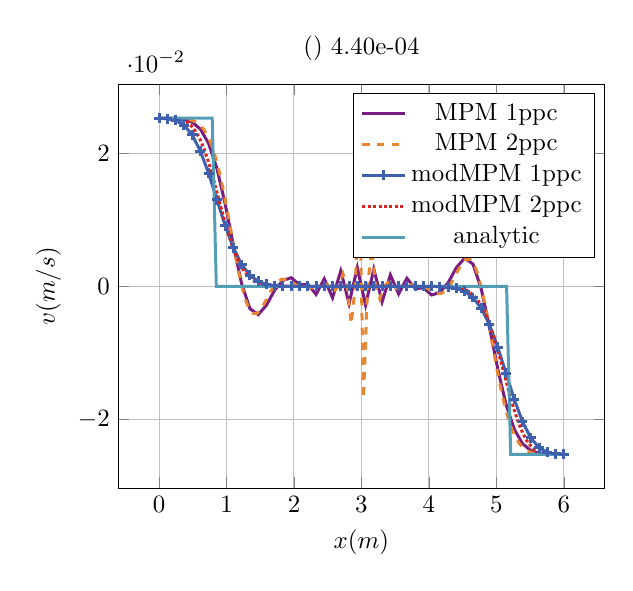
\begin{tikzpicture}[scale=0.9]
\begin{axis}[xlabel=$x (m)$,ylabel=$v (m/s)$,ymajorgrids=true,xmajorgrids=true,title={() 4.40e-04}]
\addplot[Purple,very thick,mark=none,solid] coordinates {(0.0,0.0253179577559) (0.122448979592,0.0253125244526) (0.244897959184,0.0252804932478) (0.367346938776,0.0251489907367) (0.489795918367,0.0247341796044) (0.612244897959,0.0236864809647) (0.734693877551,0.0215118739395) (0.857142857143,0.0177671095652) (0.979591836735,0.0124121755247) (1.10204081633,0.00614683940753) (1.22448979592,0.000373716046882) (1.34693877551,-0.0033616057723) (1.4693877551,-0.00426176674269) (1.59183673469,-0.00283406587609) (1.71428571429,-0.00055562049587) (1.83673469388,0.000901404345798) (1.95918367347,0.00130403292578) (2.08163265306,0.000214501074535) (2.20408163265,0.000352209313776) (2.32653061224,-0.00121718822558) (2.44897959184,0.00114054029809) (2.57142857143,-0.00172149525556) (2.69387755102,0.002335373076) (2.81632653061,-0.00259610029814) (2.9387755102,0.00282071480229) (3.0612244898,-0.00282071480229) (3.18367346939,0.00259610029814) (3.30612244898,-0.002335373076) (3.42857142857,0.00172149525556) (3.55102040816,-0.00114054029809) (3.67346938776,0.00121718822558) (3.79591836735,-0.000352209313776) (3.91836734694,-0.000214501074535) (4.04081632653,-0.00130403292578) (4.16326530612,-0.000901404345798) (4.28571428571,0.00055562049587) (4.40816326531,0.00283406587609) (4.5306122449,0.00426176674269) (4.65306122449,0.0033616057723) (4.77551020408,-0.000373716046882) (4.89795918367,-0.00614683940753) (5.02040816327,-0.0124121755247) (5.14285714286,-0.0177671095652) (5.26530612245,-0.0215118739395) (5.38775510204,-0.0236864809647) (5.51020408163,-0.0247341796044) (5.63265306122,-0.0251489907367) (5.75510204082,-0.0252804932478) (5.87755102041,-0.0253125244526) (6.0,-0.0253179577559) };
\addplot[Orange,very thick,mark=none,dashed] coordinates {(0.0,0.0253184113784) (0.0606060606061,0.0253182657812) (0.121212121212,0.0253171343813) (0.181818181818,0.0253150171787) (0.242424242424,0.0253062460446) (0.30303030303,0.0252908209787) (0.363636363636,0.0252461773758) (0.424242424242,0.0251723152357) (0.484848484848,0.0250062868064) (0.545454545455,0.024748092088) (0.606060606061,0.0242720385643) (0.666666666667,0.0235781262352) (0.727272727273,0.0224951335769) (0.787878787879,0.0210230605893) (0.848484848485,0.0190428242456) (0.909090909091,0.0165544245458) (0.969696969697,0.0136460768618) (1.0303030303,0.0103177811934) (1.09090909091,0.00694923058708) (1.15151515152,0.00354042504293) (1.21212121212,0.000626561316633) (1.27272727273,-0.00179236059183) (1.33333333333,-0.00336301978655) (1.39393939394,-0.00408541626753) (1.45454545455,-0.00406554257142) (1.51515151515,-0.00330339869822) (1.57575757576,-0.00229577774705) (1.63636363636,-0.00104267971791) (1.69696969697,-3.93881478233e-05) (1.75757575758,0.000714096963215) (1.81818181818,0.00107591385411) (1.87878787879,0.00104606252486) (1.93939393939,0.000832069940855) (2.0,0.000433936102092) (2.06060606061,0.000100491892604) (2.12121212121,-0.000168262687611) (2.18181818182,-0.000281962807299) (2.24242424242,-0.00024060846646) (2.30303030303,-0.00019473430746) (2.36363636364,-0.000144340330301) (2.42424242424,1.03021847971e-05) (2.48484848485,0.000269193237834) (2.54545454545,7.43373654573e-05) (2.60606060606,-0.000574265432333) (2.66666666667,2.52212025898e-05) (2.72727272727,0.00187279727022) (2.78787878788,-1.7779131944e-05) (2.84848484848,-0.00564650800392) (2.90909090909,-1.60332856532e-05) (2.9696969697,0.0168736450228) (3.0303030303,-0.0168736450228) (3.09090909091,1.60332856532e-05) (3.15151515152,0.00564650800392) (3.21212121212,1.7779131944e-05) (3.27272727273,-0.00187279727022) (3.33333333333,-2.52212025898e-05) (3.39393939394,0.000574265432333) (3.45454545455,-7.43373654573e-05) (3.51515151515,-0.000269193237834) (3.57575757576,-1.03021847971e-05) (3.63636363636,0.000144340330301) (3.69696969697,0.00019473430746) (3.75757575758,0.00024060846646) (3.81818181818,0.000281962807299) (3.87878787879,0.000168262687611) (3.93939393939,-0.000100491892604) (4.0,-0.000433936102092) (4.06060606061,-0.000832069940855) (4.12121212121,-0.00104606252486) (4.18181818182,-0.00107591385411) (4.24242424242,-0.000714096963215) (4.30303030303,3.93881478233e-05) (4.36363636364,0.00104267971791) (4.42424242424,0.00229577774705) (4.48484848485,0.00330339869822) (4.54545454545,0.00406554257142) (4.60606060606,0.00408541626753) (4.66666666667,0.00336301978655) (4.72727272727,0.00179236059183) (4.78787878788,-0.000626561316633) (4.84848484848,-0.00354042504293) (4.90909090909,-0.00694923058708) (4.9696969697,-0.0103177811934) (5.0303030303,-0.0136460768618) (5.09090909091,-0.0165544245458) (5.15151515152,-0.0190428242456) (5.21212121212,-0.0210230605893) (5.27272727273,-0.0224951335769) (5.33333333333,-0.0235781262352) (5.39393939394,-0.0242720385643) (5.45454545455,-0.024748092088) (5.51515151515,-0.0250062868064) (5.57575757576,-0.0251723152357) (5.63636363636,-0.0252461773758) (5.69696969697,-0.0252908209787) (5.75757575758,-0.0253062460446) (5.81818181818,-0.0253150171787) (5.87878787879,-0.0253171343813) (5.93939393939,-0.0253182657812) (6.0,-0.0253184113784) };
\addplot[Blue,very thick,mark=+,solid] coordinates {(0.0,0.0253092803388) (0.122448979592,0.0252447324562) (0.244897959184,0.0249883092861) (0.367346938776,0.0242884039338) (0.489795918367,0.0228251885418) (0.612244897959,0.0203815104479) (0.734693877551,0.0170009533921) (0.857142857143,0.0130691188281) (0.979591836735,0.00915154944222) (1.10204081633,0.00579708129579) (1.22448979592,0.00329261988393) (1.34693877551,0.001675771205) (1.4693877551,0.000752811727213) (1.59183673469,0.000303721307352) (1.71428571429,0.000103656250171) (1.83673469388,3.39292027744e-05) (1.95918367347,7.64630747692e-06) (2.08163265306,2.06351249066e-06) (2.20408163265,1.16478529579e-06) (2.32653061224,-1.70580325334e-06) (2.44897959184,2.73380703211e-06) (2.57142857143,-3.60718467272e-06) (2.69387755102,4.34097653715e-06) (2.81632653061,-4.866205363e-06) (2.9387755102,5.14034587124e-06) (3.0612244898,-5.14034587122e-06) (3.18367346939,4.86620536301e-06) (3.30612244898,-4.34097653714e-06) (3.42857142857,3.60718467272e-06) (3.55102040816,-2.73380703212e-06) (3.67346938776,1.70580325334e-06) (3.79591836735,-1.1647852958e-06) (3.91836734694,-2.06351249067e-06) (4.04081632653,-7.64630747692e-06) (4.16326530612,-3.39292027744e-05) (4.28571428571,-0.000103656250171) (4.40816326531,-0.000303721307352) (4.5306122449,-0.000752811727213) (4.65306122449,-0.001675771205) (4.77551020408,-0.00329261988393) (4.89795918367,-0.00579708129579) (5.02040816327,-0.00915154944222) (5.14285714286,-0.0130691188281) (5.26530612245,-0.0170009533921) (5.38775510204,-0.0203815104479) (5.51020408163,-0.0228251885418) (5.63265306122,-0.0242884039338) (5.75510204082,-0.0249883092861) (5.87755102041,-0.0252447324562) (6.0,-0.0253092803388) };
\addplot[Red,very thick,mark=none,densely dotted] coordinates {(0.0,0.025317930571) (0.0606060606061,0.0253168233587) (0.121212121212,0.025309085386) (0.181818181818,0.0252947166528) (0.242424242424,0.025244614182) (0.30303030303,0.0251587779735) (0.363636363636,0.0249586620152) (0.424242424242,0.0246442663072) (0.484848484848,0.0240900542943) (0.545454545455,0.0232960259765) (0.606060606061,0.0221613724279) (0.666666666667,0.0206860936486) (0.727272727273,0.0188976424995) (0.787878787879,0.0167960189808) (0.848484848485,0.0145640565488) (0.909090909091,0.0122017552037) (0.969696969697,0.00995104414047) (1.0303030303,0.00781192335918) (1.09090909091,0.00595010149482) (1.15151515152,0.0043655785474) (1.21212121212,0.00308784304074) (1.27272727273,0.00211689497486) (1.33333333333,0.00138335842096) (1.39393939394,0.000887233379031) (1.45454545455,0.000532919503373) (1.51515151515,0.000320416793985) (1.57575757576,0.000175908565338) (1.63636363636,9.9394817433e-05) (1.69696969697,4.95526747861e-05) (1.75757575758,2.63821373972e-05) (1.81818181818,1.18516742131e-05) (1.87878787879,5.96128523387e-06) (1.93939393939,2.39032827724e-06) (2.0,1.13880334319e-06) (2.06060606061,4.02762467657e-07) (2.12121212121,1.82205650633e-07) (2.18181818182,5.59845952598e-08) (2.24242424242,2.40993015384e-08) (2.30303030303,6.30122659173e-09) (2.36363636364,2.59037041968e-09) (2.42424242424,5.63023261104e-10) (2.48484848485,2.19185115995e-10) (2.54545454545,3.64413285486e-11) (2.60606060606,1.47918987648e-11) (2.66666666667,2.77206554821e-12) (2.72727272727,3.81828898731e-13) (2.78787878788,-5.09478618351e-13) (2.84848484848,9.81429969629e-14) (2.90909090909,3.0146416412e-13) (2.9696969697,1.0048488312e-13) (3.0303030303,-1.0049327836e-13) (3.09090909091,-3.01470320321e-13) (3.15151515152,-9.81477669985e-14) (3.21212121212,5.09474381606e-13) (3.27272727273,-3.81829967413e-13) (3.33333333333,-2.77206081406e-12) (3.39393939394,-1.47918927817e-11) (3.45454545455,-3.64413258703e-11) (3.51515151515,-2.19185116207e-10) (3.57575757576,-5.63023263793e-10) (3.63636363636,-2.59037042418e-09) (3.69696969697,-6.30122659737e-09) (3.75757575758,-2.40993015455e-08) (3.81818181818,-5.59845952685e-08) (3.87878787879,-1.8220565064e-07) (3.93939393939,-4.02762467661e-07) (4.0,-1.1388033432e-06) (4.06060606061,-2.39032827725e-06) (4.12121212121,-5.96128523387e-06) (4.18181818182,-1.18516742131e-05) (4.24242424242,-2.63821373972e-05) (4.30303030303,-4.95526747861e-05) (4.36363636364,-9.9394817433e-05) (4.42424242424,-0.000175908565338) (4.48484848485,-0.000320416793985) (4.54545454545,-0.000532919503373) (4.60606060606,-0.000887233379031) (4.66666666667,-0.00138335842096) (4.72727272727,-0.00211689497486) (4.78787878788,-0.00308784304074) (4.84848484848,-0.0043655785474) (4.90909090909,-0.00595010149482) (4.9696969697,-0.00781192335918) (5.0303030303,-0.00995104414047) (5.09090909091,-0.0122017552037) (5.15151515152,-0.0145640565488) (5.21212121212,-0.0167960189808) (5.27272727273,-0.0188976424995) (5.33333333333,-0.0206860936486) (5.39393939394,-0.0221613724279) (5.45454545455,-0.0232960259765) (5.51515151515,-0.0240900542943) (5.57575757576,-0.0246442663072) (5.63636363636,-0.0249586620152) (5.69696969697,-0.0251587779735) (5.75757575758,-0.025244614182) (5.81818181818,-0.0252947166528) (5.87878787879,-0.025309085386) (5.93939393939,-0.0253168233587) (6.0,-0.025317930571) };
\addplot[Duck,very thick,mark=none,solid] coordinates {(0.0,0.0253184841771) (0.0606060606061,0.0253184841771) (0.121212121212,0.0253184841771) (0.181818181818,0.0253184841771) (0.242424242424,0.0253184841771) (0.30303030303,0.0253184841771) (0.363636363636,0.0253184841771) (0.424242424242,0.0253184841771) (0.484848484848,0.0253184841771) (0.545454545455,0.0253184841771) (0.606060606061,0.0253184841771) (0.666666666667,0.0253184841771) (0.727272727273,0.0253184841771) (0.787878787879,0.0253184841771) (0.848484848485,0.0) (0.909090909091,0.0) (0.969696969697,0.0) (1.0303030303,0.0) (1.09090909091,0.0) (1.15151515152,0.0) (1.21212121212,0.0) (1.27272727273,0.0) (1.33333333333,0.0) (1.39393939394,0.0) (1.45454545455,0.0) (1.51515151515,0.0) (1.57575757576,0.0) (1.63636363636,0.0) (1.69696969697,0.0) (1.75757575758,0.0) (1.81818181818,0.0) (1.87878787879,0.0) (1.93939393939,0.0) (2.0,0.0) (2.06060606061,0.0) (2.12121212121,0.0) (2.18181818182,0.0) (2.24242424242,0.0) (2.30303030303,0.0) (2.36363636364,0.0) (2.42424242424,0.0) (2.48484848485,0.0) (2.54545454545,0.0) (2.60606060606,0.0) (2.66666666667,0.0) (2.72727272727,0.0) (2.78787878788,0.0) (2.84848484848,0.0) (2.90909090909,0.0) (2.9696969697,0.0) (3.0303030303,-0.0) (3.09090909091,-0.0) (3.15151515152,-0.0) (3.21212121212,-0.0) (3.27272727273,-0.0) (3.33333333333,-0.0) (3.39393939394,-0.0) (3.45454545455,-0.0) (3.51515151515,-0.0) (3.57575757576,-0.0) (3.63636363636,-0.0) (3.69696969697,-0.0) (3.75757575758,-0.0) (3.81818181818,-0.0) (3.87878787879,-0.0) (3.93939393939,-0.0) (4.0,-0.0) (4.06060606061,-0.0) (4.12121212121,-0.0) (4.18181818182,-0.0) (4.24242424242,-0.0) (4.30303030303,-0.0) (4.36363636364,-0.0) (4.42424242424,-0.0) (4.48484848485,-0.0) (4.54545454545,-0.0) (4.60606060606,-0.0) (4.66666666667,-0.0) (4.72727272727,-0.0) (4.78787878788,-0.0) (4.84848484848,-0.0) (4.90909090909,-0.0) (4.9696969697,-0.0) (5.0303030303,-0.0) (5.09090909091,-0.0) (5.15151515152,-0.0) (5.21212121212,-0.0253184841771) (5.27272727273,-0.0253184841771) (5.33333333333,-0.0253184841771) (5.39393939394,-0.0253184841771) (5.45454545455,-0.0253184841771) (5.51515151515,-0.0253184841771) (5.57575757576,-0.0253184841771) (5.63636363636,-0.0253184841771) (5.69696969697,-0.0253184841771) (5.75757575758,-0.0253184841771) (5.81818181818,-0.0253184841771) (5.87878787879,-0.0253184841771) (5.93939393939,-0.0253184841771) (6.0,-0.0253184841771) };
\legend{MPM 1ppc,MPM 2ppc,modMPM 1ppc,modMPM 2ppc,analytic}
\end{axis}
\end{tikzpicture}

  \caption{Comparison between exact, USF and USL velocities ate the end of the computation of the bars impact problem for various discretizations. Time $t=4.4 \times 10^{-4} \:s.$}
  \label{fig:mpm_velocities}
\end{figure}


We propose here an alternative way for reducing diffusion by using the DG approximation. 
The point of view adopted here is that a reduction of the domain rather than a widening of influence of material points may lead in a diminishing of the numerical diffusion. Mapping from particles to node identical to that of MPM whil nodes to particles is the same than this of PIC but element wise due to the discontinuous approximation. Since the mapping procedure of \cite{PIC_Nishiguchi} has been identified to be responsible for oscillations \cite{Mass_Flip}

%%% Local Variables: 
%%% mode: latex
%%% TeX-master: "../mainManuscript"
%%% End:
